\section{Related work}
Generative models, particularly in the field of machine learning and artificial intelligence, have gained substantial attention due to their capability to synthesize data that resembles real-world examples. However, the indiscriminate use of generative models can lead to undesirable consequences, such as generating biased or unreliable data. Our research aims to investigate the connection between inductive bias, rooted in domain specific knowledge, and the interpretability of generative models. By studying a diverse set of problems in the field of materials science we explore a specific category of 2D materials known as Transition Metal Dichalcogenides (TMDCs) and build digital twins for storage systems.
%%%%%%%%%%%%%%%%%

Most scientific laws are formulated to solve forward problems; they predict the properties of a system given its initial conditions. In contrast, inverse problems involve inferring the underlying causes, factors, or structures responsible for a set of observations. These problems arise in two key contexts. In the first case,  inverse problems are solved to deduce physical laws, relations, or a humble parameter value from the experimental data. In the second, we put scientific knowledge to practical use and create an object with the desired properties. Attempts to solve inverse problems have been undertaken in a wide range of fields: engineering, material science, non-destructive testing, geophysics, radiation therapy, computational fluid dynamics, medical imaging, geology, astronomy, and economics.\todo{references?}

Over the last decade, remarkable progress in material science has been achieved, significantly pushing forward many applications, from electronics to energy, composite materials to membranes. Consequently, the development of materials with predetermined properties has become critical for numerous critical technologies.

The inverse problem in material science arises in many different areas, from mechanics to the atomic structure of materials, from spectroscopy data analysis to material design \cite{Lionheart2007Analysis, molesky2018inverse, zunger2018inverse, long2021constrained, Ren2021Invertible}. This article focuses on a specific facet: determining the composition and structure of a 2D crystal based on its macroscopic physical properties, such as strength, elasticity, conductivity, \emph{etc}.

Material discovery is a complex process with a general workflow that can be broken down into several parts, as depicted in Figure~\ref{fig:introduction:design-workflow}. Firstly, new material candidates are generated, and their suitability for potential applications is simulated. Next, the material with the highest likelihood of success is synthesized. Lastly, the material is incorporated into a device and its desired properties are investigated. The time required to design a material is thus dependent on three factors: (i) the number and duration of simulations, (ii) the duration of synthesis of proposed candidates, and (iii) the time needed for measurements and the selection of the best candidates. The usual material's discovery or optimization time is measured in years \cite{maine2016accelerating} and requires significant human and computational resources. The inverse design approach aims to accelerate the process of discovery of new materials by efficiently and accurately finding candidates in silico.
\begin{figure}[htp]
    \noindent
    \centering
    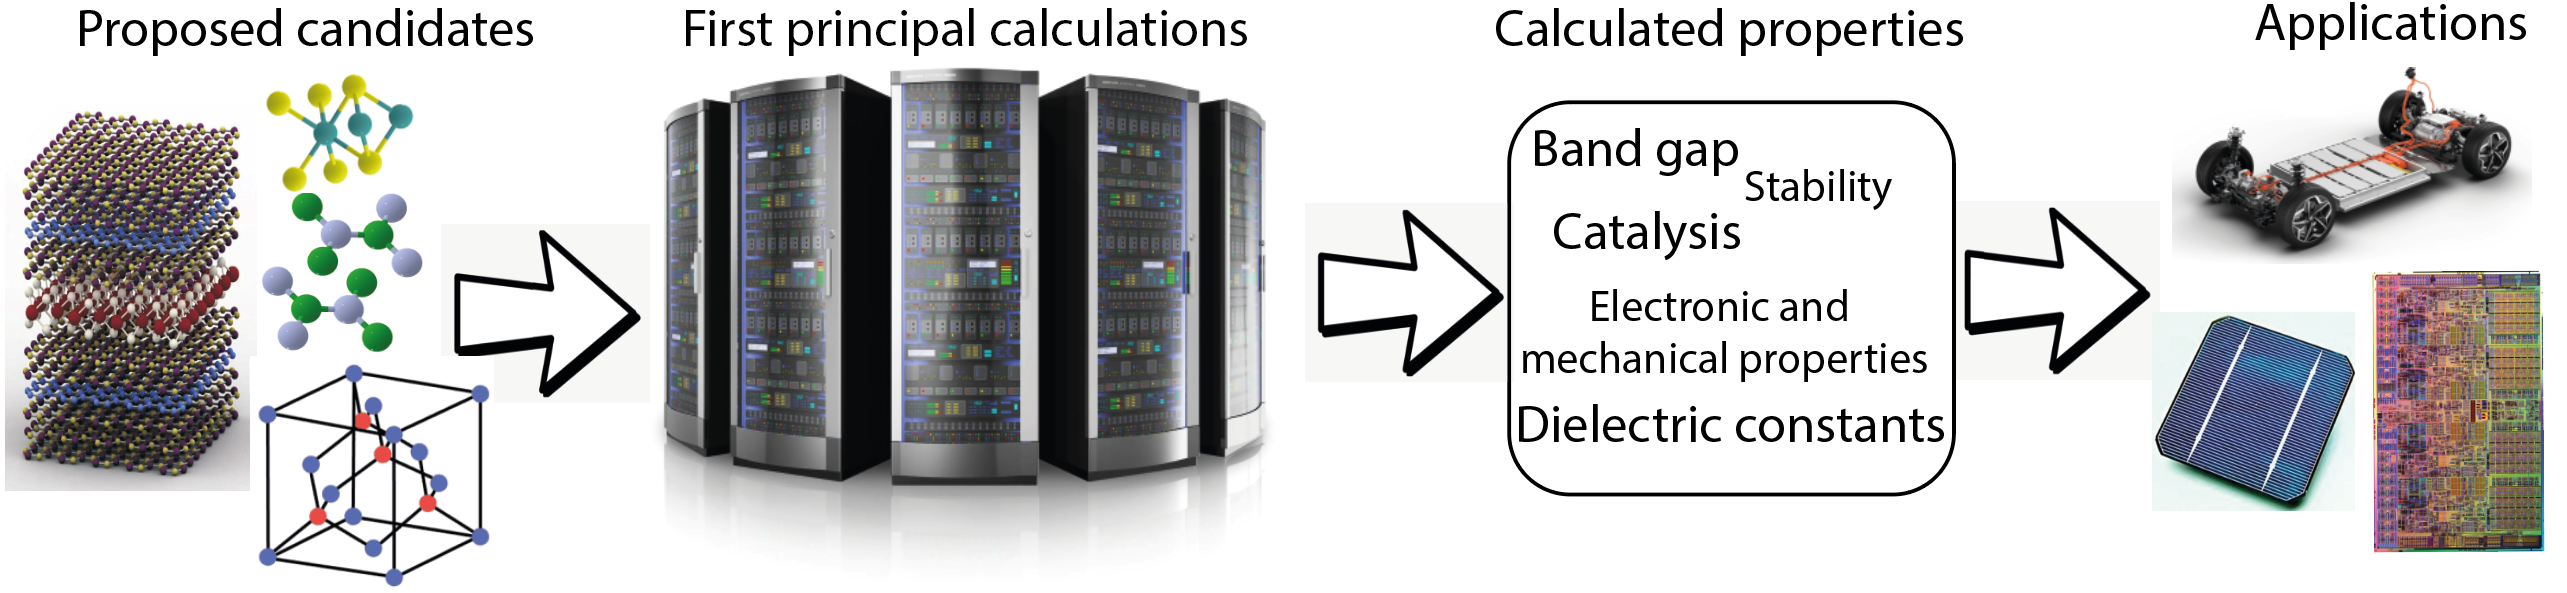
\includegraphics[width=\textwidth]{figures/Discovery_pipe.png}
    \caption{The classical material design workflow. Candidate materials are intuitively perceived and their properties are computed in silico and verified experimentally.}
    \label{fig:introduction:design-workflow}
\end{figure}

A schematic overview of material design problems and their possible solutions is presented in Figure~\ref{fig:property-space}, where we link the material space and the material functional space. 


This chapter is structured as follows. In subsection \ref{subsec:forward:physics}, we discuss the simulation of materials based on physical principles; in subsection~\ref{subsec:Atomic} we review structure representations suited for machine learning; in subsection~\ref{subsec:forward:ml} -- property prediction based on machine learning. Section \ref{sec:inverse} is dedicated to the inverse problem; in subsection~\ref{subsec:High-throughput} we cover high-throughput virtual screening technique; in subsection~\ref{subsec:Evolutionary} -- evolutionary design methods; in subsection~\ref{subsec:intelligence} -- generative machine learning methods; in subsection~\ref{subsec:Reinforcement} -- the recent applications of the reinforcement learning approach. Section \ref{sec:Discussion} concludes the paper with a discussion of the methods' applicability and general outlook. \todo{consider reformatting the paragraph}

\begin{figure}[H]
	\noindent
	\centering
	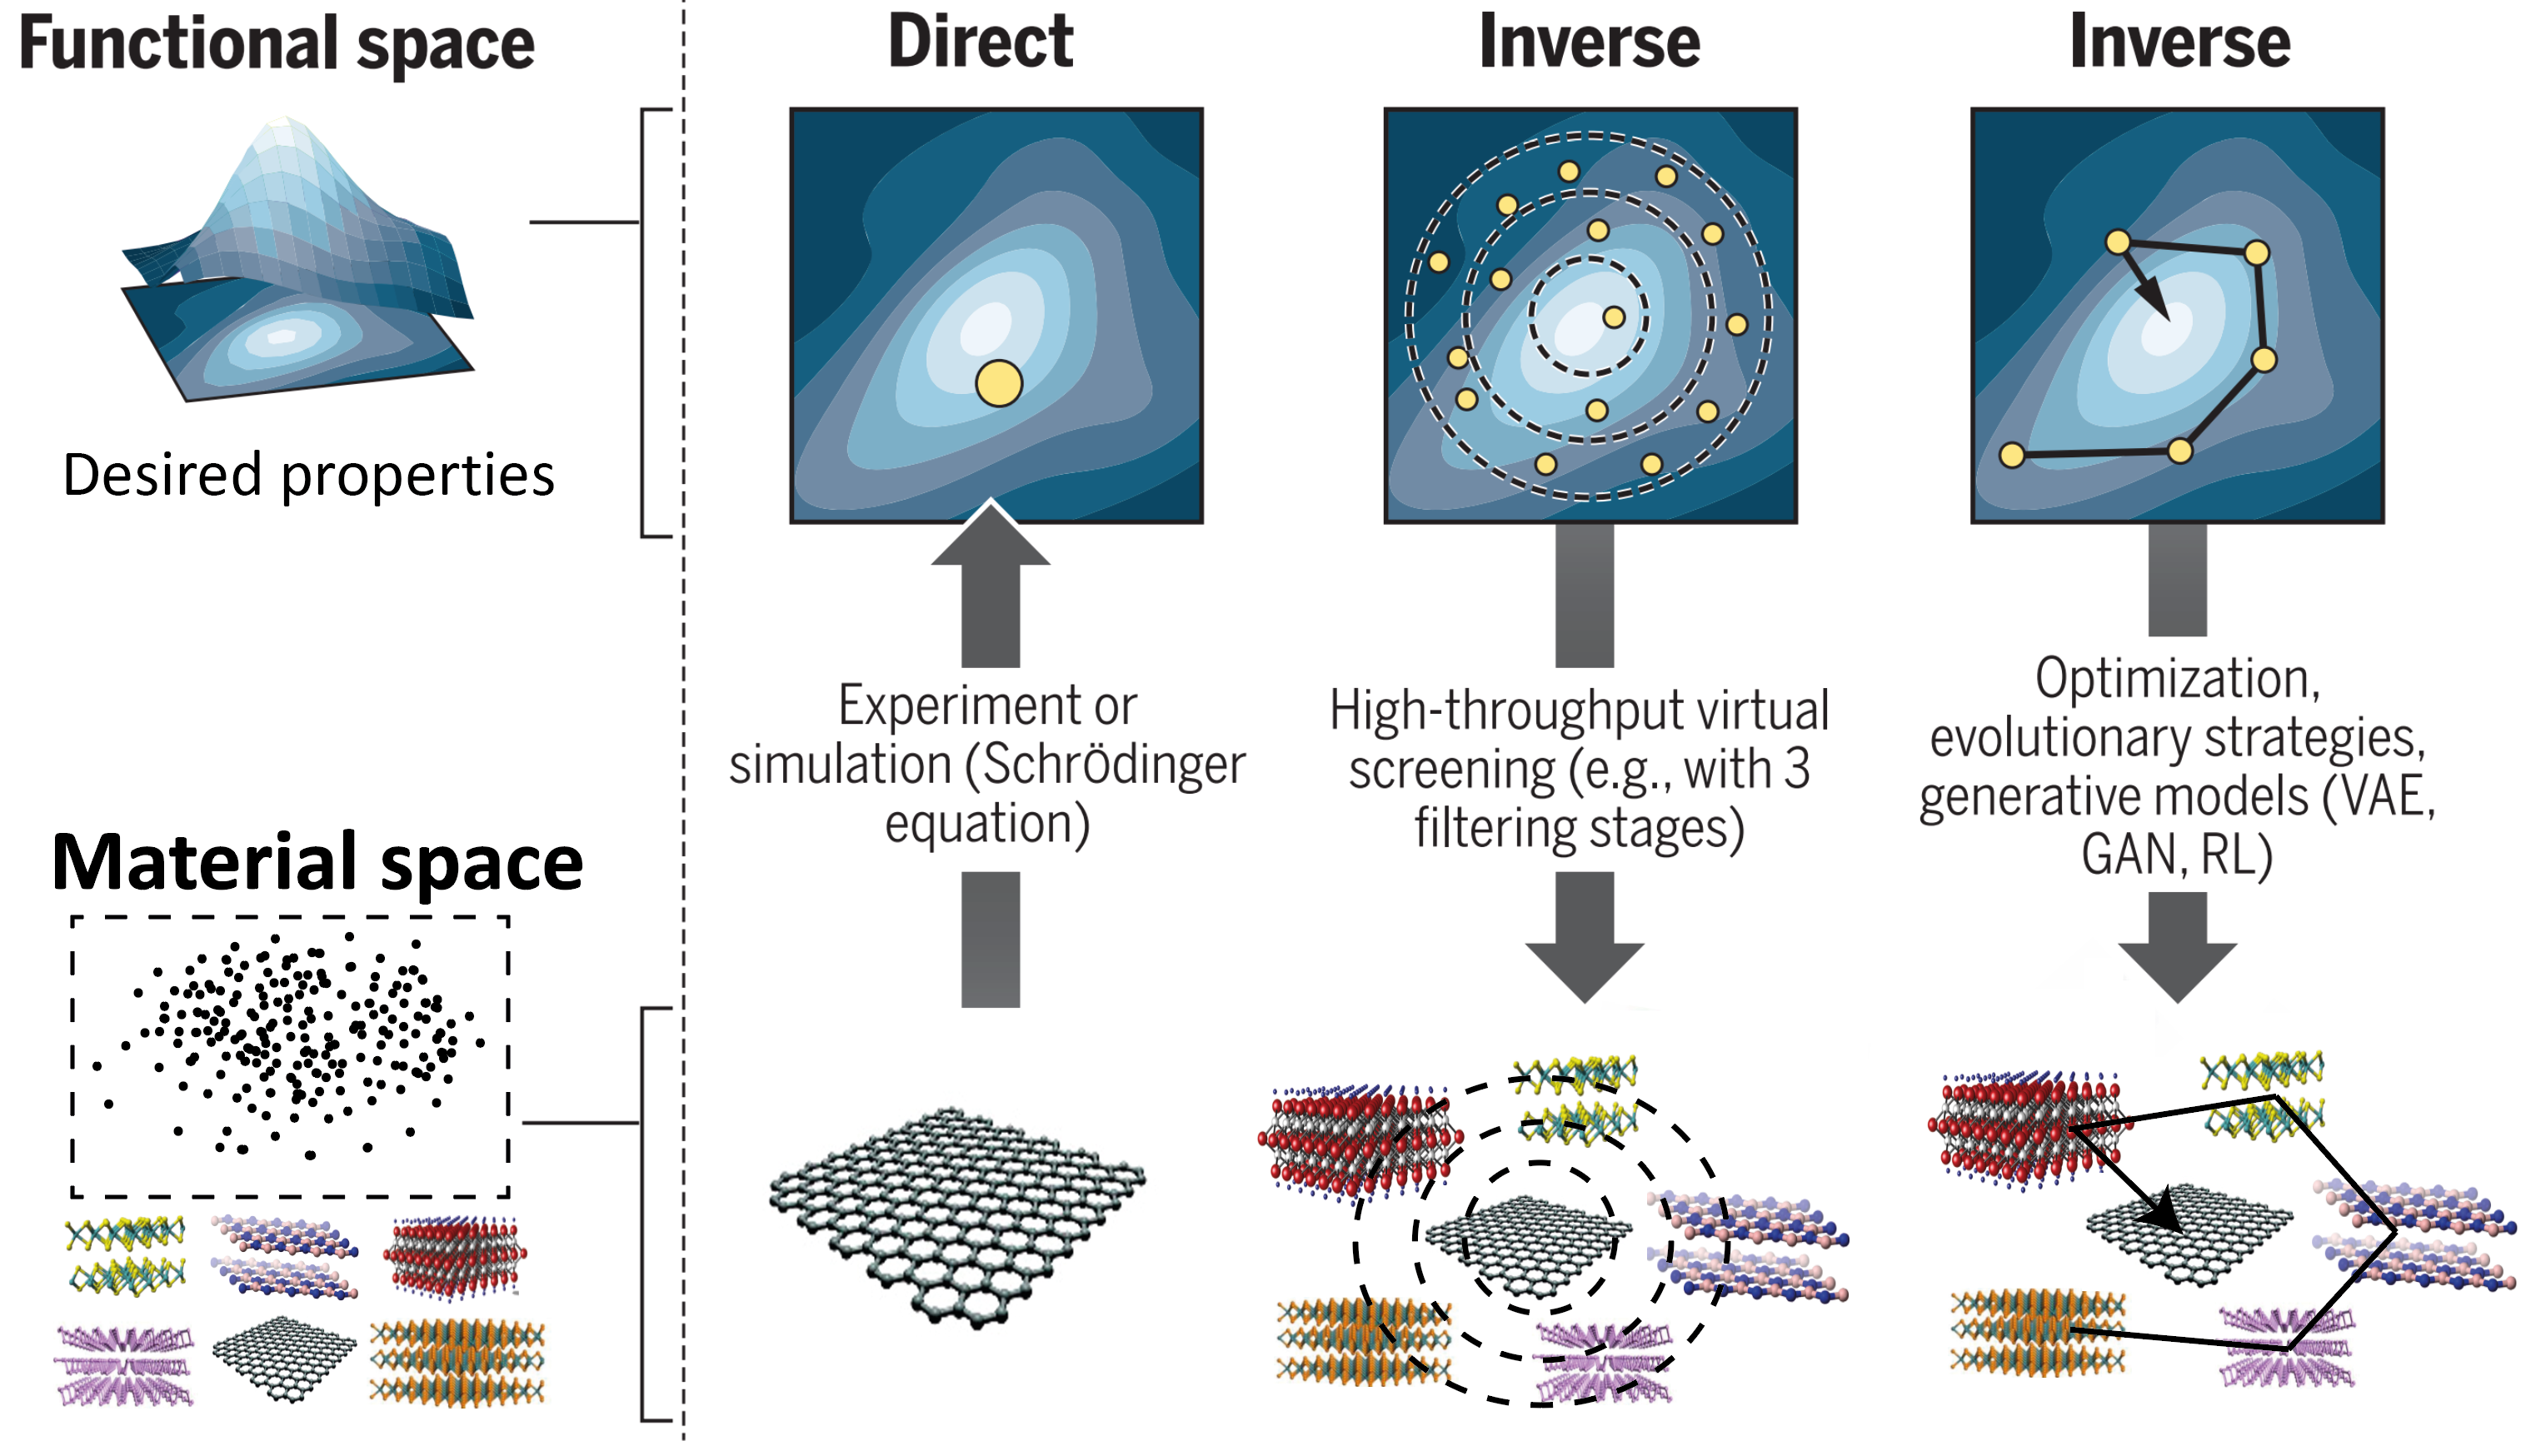
\includegraphics[width=\textwidth]{figures/Property_space_3.png}
	\caption{ Schematic illustration of material and functional space and different approaches toward materials design. Adapted from \cite{sanchez2018inverse}}
	\label{fig:property-space}
\end{figure}

\subsection{Material simulation}
\label{sec:forward}
\subsubsection{Ab-initio methods}
\label{subsec:forward:physics}
In the 20th century, the formulation of quantum mechanics solved the principal problem of theoretical atomic systems description. However, the many-body Schrodinger equation is too complex to be directly solved for most real-world systems. Hence, a number of approximate methods was developed. One of the most widely used approaches for materials is density functional theory (DFT)~\cite{parr1980density}. It allows for relatively efficient calculation of the electron ground state and its properties, such as the energy and the band structure. DFT has been used to generate large material databases \cite{choudhary2022recent} and to train machine learning algorithms \cite{schleder2019dft}. The computation time of DFT is proportional to the cube of the number of atoms in the structure \cite{burke2012perspective, pan2021scaling}, with the practical system size ceiling of around 1000 atoms. Taking advantage of the interaction locality allows the use of DFT for larger systems with computational time linearly dependent on the number of atoms~\cite{nakata2020large}, but provides little advantage for small systems. The accuracy of DFT in describing nanoscale material properties has led to its widespread adoption in various scientific software packages, a complete list of which can be found in Wikipedia\footnote{ \url{https://en.wikipedia.org/wiki/List_of_quantum_chemistry_and_solid-state_physics_software}}. 

Several DFT-derived databases cataloging an array of structures, from molecules to crystals, have been made available for diverse research objectives. We enumerate the principal online datasets in Table \ref{table:Table1}. Some of these databases contain a wide variety of structure types, including 2D materials. In Table \ref{table:Table2}, we have collected databases containing 2D materials. It is worth mentioning that a much more extensive list of datasets suitable for training machine learning algorithms to predict material properties is available\footnote{ \url{https://github.com/JuDFTteam/best-of-atomistic-machine-learning}}. Despite the breadth of these resources, the exhaustive landscape of materials and their properties remains incompletely mapped. This prompts ongoing efforts by research collectives to compile specialized datasets tailored to specific investigational needs \cite{lu2024machine}.

\begin{table}[ht]
    
    \centering
    \begin{tabular}{l l l l}
        \toprule
        \hline
        Dataset      & Size   & URL   \\
        \hline
        QM7, QM7b, QM8, &&& \\
        QM7bml, QM9, QM7-X & $ >100k$ & \url{http://quantum-machine.org/}  \\
        Alchemy &  200K & \url{https://alchemy.tencent.com/}  \\
        ANI-1 & 20M &  \url{https://github.com/isayev/ANI1_dataset} \\
        ANI-1x & 5M &  \url{https://github.com/aiqm/ANI1x_datasets} \\
        AGZ7 & 140k & \url{https://github.com/binghuang2018/agz7} \\
        tmQM & 80k & \url{https://github.com/bbskjelstad/tmqm} \\
        OQMD & $>1M$ & \url{https://oqmd.org/} \\
        The Open Catalyst & $>1M$ & \url{https://opencatalystproject.org/&} \\
        AFlow & 3.5M & \url{https://www.aflowlib.org/} \\
        Materials Project & $>600k$ & \url{https://www.materialsproject.org} \\
        Materials Cloud & $>10M$ & \url{https://www.materialscloud.org/home} \\
        \bottomrule
        
    \end{tabular}
    \caption{Generic material datasets.}
    \label{table:Table1}
\end{table}

\begin{table}[ht]
    \centering
    \begin{tabular} {l l l l}
        \toprule
        \hline
        Dataset   & Size   & URL  \\
        \hline
        Aflow & 3.5M & \url{https://www.aflowlib.org/} \\
        JARVIS-DFT & 77k & \url{https://jarvis.nist.gov/} \\
        C2DB & 4k & \url{https://www.cmr.fysik.dtu.dk/c2db/c2db.html} \\
        aNANt &23k& \url{https://www.anant.mrc.iisc.ac.in} \\
        Materials Cloud & $>10M$ & \url{https://www.materialscloud.org/home} \\
        2DMatPedia& 6k & \url{http://www.2dmatpedia.org/} \\
        Materials Project & $>600k$&  \url{https://www.materialsproject.org} \\
        ICSD &300k & \url{https://www.psds.ac.uk/icsd} \\
        COD &500k & \url{https://www.crystallography.net/cod/} \\
        CSD & 1M & \url{https://www.ccdc.cam.ac.uk/} \\
        OQMD  &300k& \url{https://oqmd.org/} \\
        QPOD &2k& \url{https://cmr.fysik.dtu.dk/qpod/qpod.html} \\
        2DMD  &$>15k$& \url{https://rolos.com/open/2d-materials-point-defects/} \\
        2D Materials  & 6k &  \url{https://cmr.fysik.dtu.dk/c2db/c2db.html} \\
        \bottomrule
    \end{tabular}
    \caption{Crystal structures datasets with 2D materials.}
    \label{table:Table2}
\end{table}

The exploration of large atomic systems with more than a thousand atoms is predominantly facilitated through Molecular Dynamics (MD) simulations. In MD, atoms are treated as classical particles that interact with each other; classical MD deals with only forces, energies, and stress -- without simulating electrons in any way. It is a very powerful set of methods for predicting mechanical properties. In a simple case, MD uses heuristic interatomic interaction potentials (EIP); providing a computationally efficient means to simulate systems comprising up to $10^{6}$ atoms. However, widely used set of interatomic simulations like Tersoff \cite{tersoff1989modeling}, AIREBO \cite{stuart2000reactive}, ReaxFF \cite{srinivasan2015development}, and optimized Tersoff \cite{lindsay2010optimized} can fail in seemingly straightforward simulations, such as those involving graphene \cite{mortazavi2021first}. Each atomic system needs carefully selected inter-atomic potential and its parameters. Ab initio MD (AIMD) overcomes this issue by mixing DFT and MD, but these methods are limited by computational cost since they rely on DFT.
 
Since the interatomic interaction potentials are by their nature heuristic approximations, machine learning has been systematically and successfully used to train ML interatomic potentials (MLIP) on the DFT data, starting with~\cite{behler2007generalized}. Modern methods~\cite{mortazavi2023atomistic, anstine2023machine, wen2022deep} provide accuracy comparable to DFT with EIP computational speed. Now MLIPs can be used in MD simulations using either generic packages like LAMMPS~\cite{LAMMPS}, as well as within specialized packages like TorchMD~\cite{doerr2020torchmd} and DeepMD~\cite{wang2018deepmd}. Nowadays MLIPs are greatly used in material simulations, acceleration of materials design \cite{gubaev2019accelerating,podryabinkin2019accelerating, lu202186}, and predicting material properties \cite{mortazavi2020exploring}. There are few types of MLIPs: neural network potentials (NNPs) \cite{behler2007generalized,chen2022universal,wen2022deep}, Gaussian approximation potentials (GAPs) based on Gaussian process regression \cite{bartok2010gaussian}, moment tensor potentials (MTPs) \cite{novikov2020mlip,shapeev2016moment}, spectral neighbor analysis potentials (SNAPs) \cite{thompson2015spectral}, deep tensor neural networks \cite{schutt2017quantum}, Gaussian moment neural network potentials (GM-NNPs) \cite{zaverkin2020gaussian} and most recently neuroevolution-potentials (NEPs) \cite{fan2021neuroevolution}. In comparison to EP, MLIPs, as other ML methods, rely heavily on the quality and diversity of training data, trained using DFT-based datasets in combination with AIMD data, including high-temperature regimes, to take into account diverse atomic environments. Temperature effects represent a huge niche where MLIPs are found to be more accurate than traditional DFT and EP \cite{mortazavi2023atomistic}. MLIPs have shown particular promise in the research of two-dimensional (2D) materials. For instance, they have been applied to study 2D lattices of biphenylene \cite{fan2021biphenylene}, quasi-hexagonal-phase \ce{C_{60}} fullerene (\ce{qHPC_{60}}) \cite{hou2022synthesis}, \ce{BC_2N} \cite{seo2021dominant}, \ce{MoS_2} \cite{marmolejo2022thermal}.

\subsubsection{Atomic structure representation}
\label{subsec:Atomic}

\begin{figure}[htp]
    \noindent
    \centering
    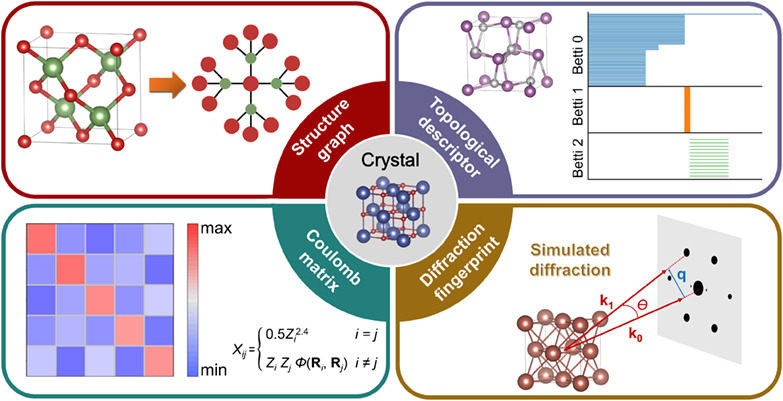
\includegraphics[width=\textwidth]{figures/Crystal_representation.jpg}
    \caption{One crystal can be represented in various ways using different representations. These representations include: a graph containing atom and bond weights, Coulomb matrix,   diffraction fingerprint, using topological descriptors and etc. Taken from \cite{li2022encoding} with permission.}
    \label{fig:representations}
\end{figure}

The core problem of building a model of a given structure is the mathematical representation of an atomic system. Suppose we follow Born-Oppenheimer (BO) approximation and presume that the electrons are in the ground state. In that case, the atomic system is fully described as a set of atoms, their positions, and momenta. Using the raw coordinate values as algorithm input is counterproductive as this doesn't respect the rotation, translation, and permutation equivariance and quickly leads to a problem of intractable computational complexity. A good representation must respect those symmetries. There are two observations that are usually useful when constructing such representations. Firstly, most atomic-scale properties are continuous and smooth functions of the atomic coordinates. Representations that preserve this smoothness are preferred. Secondly, representation usually loses a certain amount of information. Discarded information might limit the accuracy of the model. 

Early interatomic interaction potentials used just the pairwise distances~\cite{jones1924determination} to compute pairwise forces. While conceptually simple and computationally efficient, this approach can not describe complex interactions. More advanced descriptors were primarily based on fingerprints driven by chemical intuition \cite{Burden2009Toward, Dong2015ChemDes, Winter2018Learning, wale2007comparison}, and molecular and crystal graphs \cite{Jiang2021CouplingCS, Singh2022MathematicalAO, Jiang2021AUD,Balasingham2022CompactGR}. Modern empirical interatomic potentials \cite{Shui2022InjectingDK, Rohskopf2017EmpiricalIP, Ito2016SystematicAT, Shui2022InjectingDK} are typically expressed as an additive combination of local terms and long-range pairwise contributions. Hence, additive, atom-centered representations have become popular in molecular machine learning. 

Other possible material representations include structure fingerprints \cite{warr2011representation}, inspired by the Fourier transform Diffraction fingerprints \cite{ziletti2018insightful}, which are widely used as crystal descriptors. Coulomb matrices \cite{tchagang2019prediction}  each element is calculated based on the Coulombic interactions between atoms. The diagonal elements reflect the properties of individual atoms, while off-diagonal elements represent interactions between different atoms. And other methods like: bags of bonds \cite{hansen2015machine}, Indicators from quantum chemical calculations \cite{Dronskowski1993CrystalOH}, Empirical valence bond (EVB) method \cite{Warshel2004TheEV}, SPRINT method \cite{PhysRevLett.107.085504}, Overlap matrix eigenvalue fingerprints \cite{PhysRevLett.107.085504, zhu_fingerprint_2016}.

Topological Descriptors \cite{li2022encoding}, particularly those based on persistent homology, are advanced tools used in materials science to encode compounds' structural information. They work by representing chemical structures as a series of interconnected points (like a 3D point cloud), capturing the structure's local and global details. 

Voxel-based representations \cite{kajita2017universal} naturally preserve translation-invariant features and provide a rich input to computer-vision inspired neural networks, but until recently~\cite{weiler2019general} suffered from the lack of a way to encode the rotation symmetry.

Graph representation of an atomic system~\cite{xie2018crystal} respects all the symmetries and also provides for interaction locality. It is used in most state-of-the-art machine learning methods. We will discuss it in more detail in the next subsection~\ref{subsec:forward:ml}.

In small organic molecules, most information about the structure can be recovered from just a graph of atoms and bonds between them. This allows grammar-based representation, exemplified by the Simplified Molecular Input Line Entry System (SMILES) \cite{doi:10.1021/ci00062a008}, to be commonly used to represent them. However, it is limited to stereochemistry types, has no standard for handling aromaticity, and no way to generate canonical representation \cite{oboyle_towards_2012}. The recent development of SELFIES \cite{krenn2022selfies} as next-generation molecule text representation has the potential to overcome some of these limitations. However, the SMILES or SELFIES methods can't be used to describe crystal structure yet because crystal representation must satisfy translational, rotational, and permutational invariances. In a recent article, the first string-based method for representing crystal structures SLICES was presented \cite{xiao2023invertible}. 

The methods mentioned here are by no means an exhaustive list. Musil et al. \cite{doi:10.1021/acs.chemrev.1c00021} provided an excellent review of the different methods used for the structure representation of molecules and crystals. The choice of representation ultimately depends on the available data. While numerous databases are readily accessible online \cite{choudhary2022recent}, 2D material datasets remain limited. However, the field is rapidly evolving with the availability of new datasets \cite{haastrup2018computational, gjerding2021recent, huang2023unveiling}, and further research is required to explore the potential of different material representations fully.

% (Nikita) a list of citations in unhelpful
% This trend has necessitated the transformation of atomic configurations into a more suitable representation in a feature space, which can then be utilized for various machine learning methods such as regression of structure-property relationships \cite{Dai2020Method, Zhang2020novel}, clustering \cite{Francia2020SystematicFR, Chisholm2005COMPACKAP}, and low-dimensional visualization of the energy landscapes \cite{doi:10.1073/pnas.1108486108}.

% TODO(Nikita) where do those models come with the respect to the other properties?
% To overcome this limitation, representations independent of atom ordering, such as permutation-invariant polynomials \cite{Oord_2020, Balan2022PermutationIR}, have been developed.

\subsubsection{Machine learning}
\label{subsec:forward:ml}



Machine intelligence or Artificial intelligence is a rapidly growing field encompassing machine learning and deep learning. Machine learning is a subfield of artificial intelligence concerned with developing algorithms and statistical models that enable computer systems to learn from data and make predictions or decisions based on that data. In contrast, deep learning is a specific subset of machine learning that uses artificial neural networks to perform tasks that require a high degree of abstraction, such as image and speech recognition, natural language processing, and the applications of other scientific domains \cite{Goodfellow-et-al-2016}. The relationship between the fields is depicted in figure~\ref{fig:forward:ml-ontology}.


%The general pipeline of constructing an AI model consists of three steps. Firstly, an Ab-initio methods is proposed that computes forces, or other quantities of interest, from the atomic structure. Secondly, a representative dataset is computed with a chosen ab initio method. Finally, AI model's parameters are fitted so match the data. Machine learning provides more expressive parameterizations that allow taking advantage of larger datasets, and active learning can help construct an optimal dataset.

While both machine learning and deep learning involve training algorithms on data to make predictions or decisions, they differ in their approach to learning and the types of problems they are best suited for. Machine learning typically relies on hand-crafted features usually designed by domain experts, reflecting their priors and inductive biases to capture the relevant information in the data. In contrast, deep learning models learn to extract relevant features directly from the data using multiple layers of interconnected nodes that can learn increasingly abstract representations of the data. Reflecting the biases and the symmetries into those layers is usually more complicated, as it requires the introduction of invariances and equivariance into the definition of the layers.

The ability of deep learning models to automate feature selection is a significant advantage over traditional machine learning methods. This advantage has been demonstrated in numerous applications, including images \cite{rombachHighResolutionImageSynthesis2022a}, speech recognition \cite{radfordRobustSpeechRecognition2022}, natural language processing \cite{brownLanguageModelsAre2020a}, game playing \cite{silverMasteringGameGo2016}, protein folding \cite{jumperHighlyAccurateProtein2021a}.  For example, in material science, deep learning models have been used to predict or classify material properties without involving hand-crafted features. Ma et al. \cite{ma2021large} used a combination of deep learning and ab initio calculations to discover novel 2D ferroelectric materials. Wilhelm et al. \cite{willhelm2022predicting} employed various DL methods to predict the physical properties of Van der Waals heterostructures from their constituent monolayer properties.

Machine learning can be broadly classified into three categories: supervised learning, unsupervised learning, and reinforcement learning. In supervised learning, a model is trained on labeled datasets of input-output pairs to learn the underlying relationship between the input and output variables. On the other hand, unsupervised learning involves training a model on an unlabeled dataset to discover patterns and structure in the data, relying on metric distances and differences between samples. Reinforcement learning is a type of learning in which an agent learns to interact with an environment to maximize a reward signal.

The development of machine intelligence has led to numerous breakthroughs in fields such as computer vision, natural language processing, and robotics. With the availability of large amounts of data and the development of powerful computing hardware, the potential of machine intelligence to revolutionize various industries and sectors is enormous. Goodfellow et al.~\cite{Goodfellow-et-al-2016} provide a comprehensive overview of machine learning and deep learning, including their classifications, applications, and challenges.
\begin{figure}[htp]
    \noindent
    \centering
    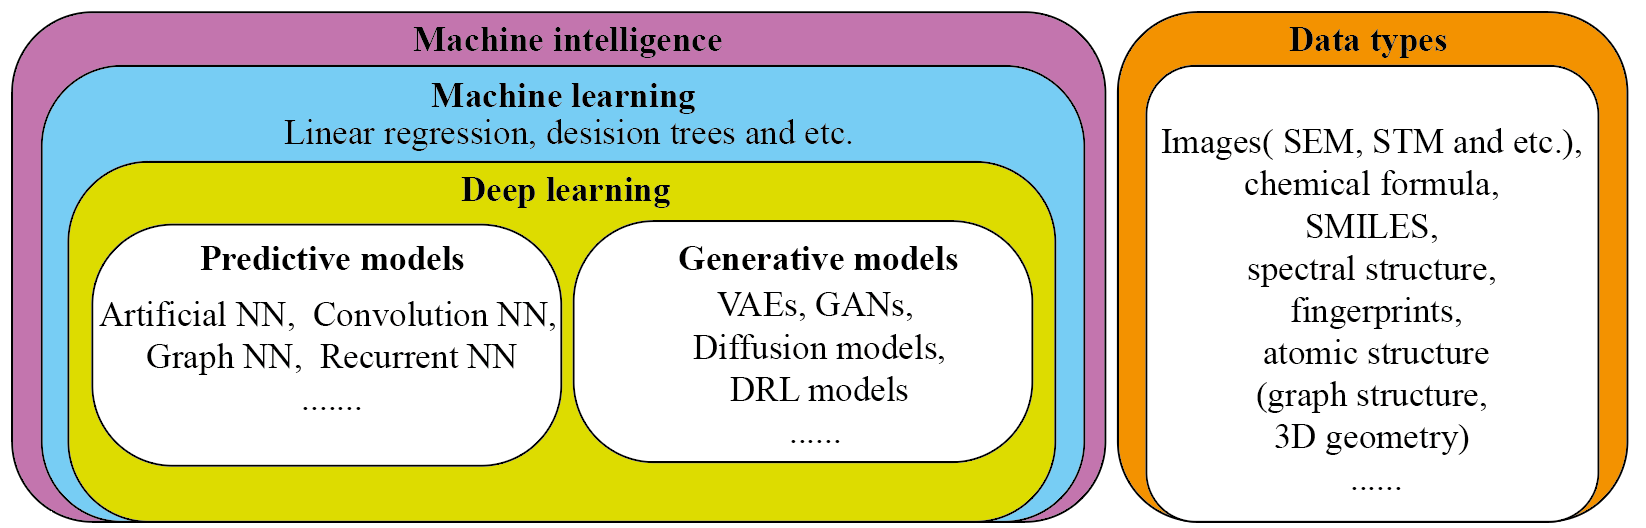
\includegraphics[width=12.6cm]{figures/Sub-fields_of_machine intelligence_3.png}
    \caption{Different sub-fields of machine intelligence.}
    \label{fig:forward:ml-ontology}
\end{figure}

In recent years, machine learning algorithms have been extensively used for predicting or classifying material properties. For instance, decision trees, support vector machines \cite{tang2010prediction,balachandran2015materials}, and other machine learning methods have been applied to 2D materials \cite{schleder2019exploring,tawfik2019efficient}. Wilhelm et al. \cite{willhelm2022predicting} employed different machine learning methods, including AdaBoost, Elastic Net, Gradient Boosted Trees, Kernel Ridge Regression, and Support Vector Regression, to predict the physical properties of Van der Waals heterostructures from their constituent monolayer properties.

\textbf{Convolution Neural Networks (CNNs)} \cite{gu2018recent}  are highly effective in deep learning, specifically for spatial data. Convolutional layers use kernels to scan the input, which is typically discretized on a grid, and the same filter is used multiple times with different positions in the input. Such parameter sharing makes training CNNs more efficient. Translation invariance is also an essential feature of convolution. It is particularly important for image processing because features such as edges and shapes can be present anywhere in the case of images; thus, convolution helps capture these features regardless of their location.

\begin{figure}[H]
    \noindent
    \centering
    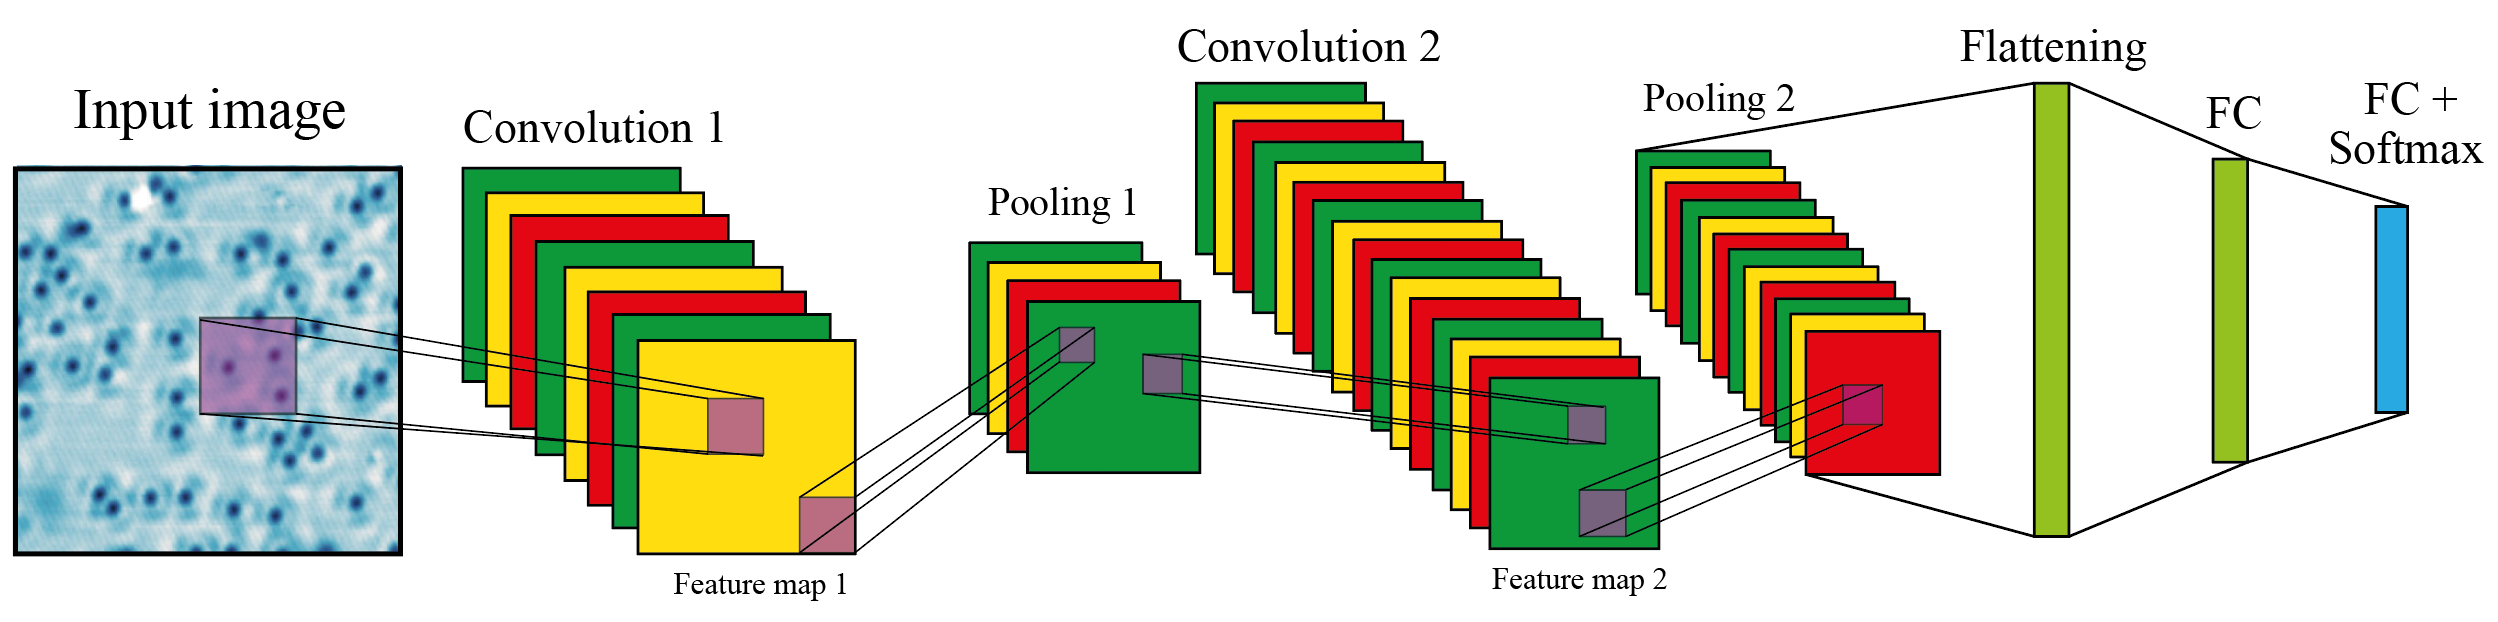
\includegraphics[width=13.6cm]{figures/CNN.png}
    \caption{Convolution Neural Network. The 2D material image from \cite{li2021ordered}}
    \label{fig:cnn}
\end{figure}

Another useful feature is local connectivity. Convolutional layers use kernels with varying spatial extent. The schematic illustration of simple CNN is presented in ~\ref{fig:cnn}. This local connectivity allows the network to capture local patterns in the structure or the image, such as edges, corners, texture in the case of images, or atom types and other physics-based descriptors e.g., structure density, volume per atom, maximum packing fraction, structural complexity \cite{PhysRevMaterials.2.083801}, XRD powder pattern \cite{LamPham2017}, orbital field matrix \cite{Ong2013}, and JarvisCFID \cite{ complexity2013}. Combining multiple convolutional layers with different filters can capture increasingly complex patterns, allowing the network to learn hierarchical representations of the input. Usually, convolutional layers are followed by pooling or reduction layers, designed to reduce the spatial resolution of the input while retaining the most important information. This helps to make the network more robust to small movements after translation translations and deformations in the input and also reduces the number of parameters that need to be learned.

The main issue with utilizing the regular CNN (where the domain of the operation is defined as a grid) for materials science is that the locations of atoms and molecules are usually not restricted to a grid, and their precise locations carry important information that will be lost if discretized to a grid. Based on that, the authors of SchNet \cite{schutt2017schnet} develop a continuous filter convolution where the input is not required to be embedded on a grid. SchNet is designed to learn a representation for predicting different physical attributes, mainly energies and atomic forces. The model is invariant with respect to translation and permutations of atom indexing, with a smooth energy prediction w.r.t. perturbation to atom positions and energy conservation of the predicted force fields. The energy and force predictions are rotationally invariant and equivariant, respectively. At the time, SchNet demonstrated state-of-the-art results on the QM9~\cite{ruddigkeit2012enumeration,ramakrishnan2014quantum} dataset and accurate results for MD17~\cite{chmiela2017machine} and ISO17~\cite{schutt2017schnet}.

\subsubsection{Graph Neural Networks}
\label{subsubsec:gnns}
Graph Neural Networks (GNNs)\cite{battagliaRelationalInductiveBiases2018, kipfSemiSupervisedClassificationGraph2017} are an important class of machine learning algorithms that operate on graph-structured data. Mathematically, a graph consists of two sets: nodes $V$ (alternatively called vertices) and edges $E$. An edge connects two vertices, hence $E\subset V^2$. A graph can have additional data associated with its elements, typically called node and edge features.

Such general and straightforward definitions make graphs a suitable mathematical model for a wide variety of data. For example, images can be presented as a graph structure with a regular grid-like structure, with individual pixels representing nodes and RGB channel values at each pixel serving as node features. CNNs have shown a great ability to extract features from image-like data. Thus, it would be natural to generalize this idea to graphs of any kind. A rectangular convolutional filter expects a fixed number of pixels as its input. The weights also depend on the relative position of the pixels. A graph, however, doesn't have a natural ordering of the neighbors and can have an arbitrary number of them. Therefore, in a graph convolution, every neighboring node participates with the same weight.

Consider a graph example inFigure~\ref{fig:gnn}(a) that can represent a small molecule. Figure~\ref{fig:gnn}(b) depicts how the two-layer classic Convolutional GNN looks like for that graph. The first layer (layer 0) consists of just node feature vectors, which serve as an input to GNN layers. For each node, we define a computational graph that differs from node to node and depends on node surroundings, but the depth is the same for all of them. Node 1~\ref{fig:gnn}(b) aggregates and processes information by a nonlinear function, which may be by itself a small NN. The information aggregation from node neighbors and neighbors of its neighbors, such aggregation is called two-hop aggregation or two layers of GNN block. Usually, there is no need to have a large number of GNN layers unless you are working with graphs of high diameter. To make GNN more expressive, the post and pre-processing layers and residual connections can be added as schematically shown in ~\ref{fig:gnn}(c). The second way to improve GNNs is to modify the GNN blocks by themselves.

\begin{figure}[H]
    \noindent
    \centering
    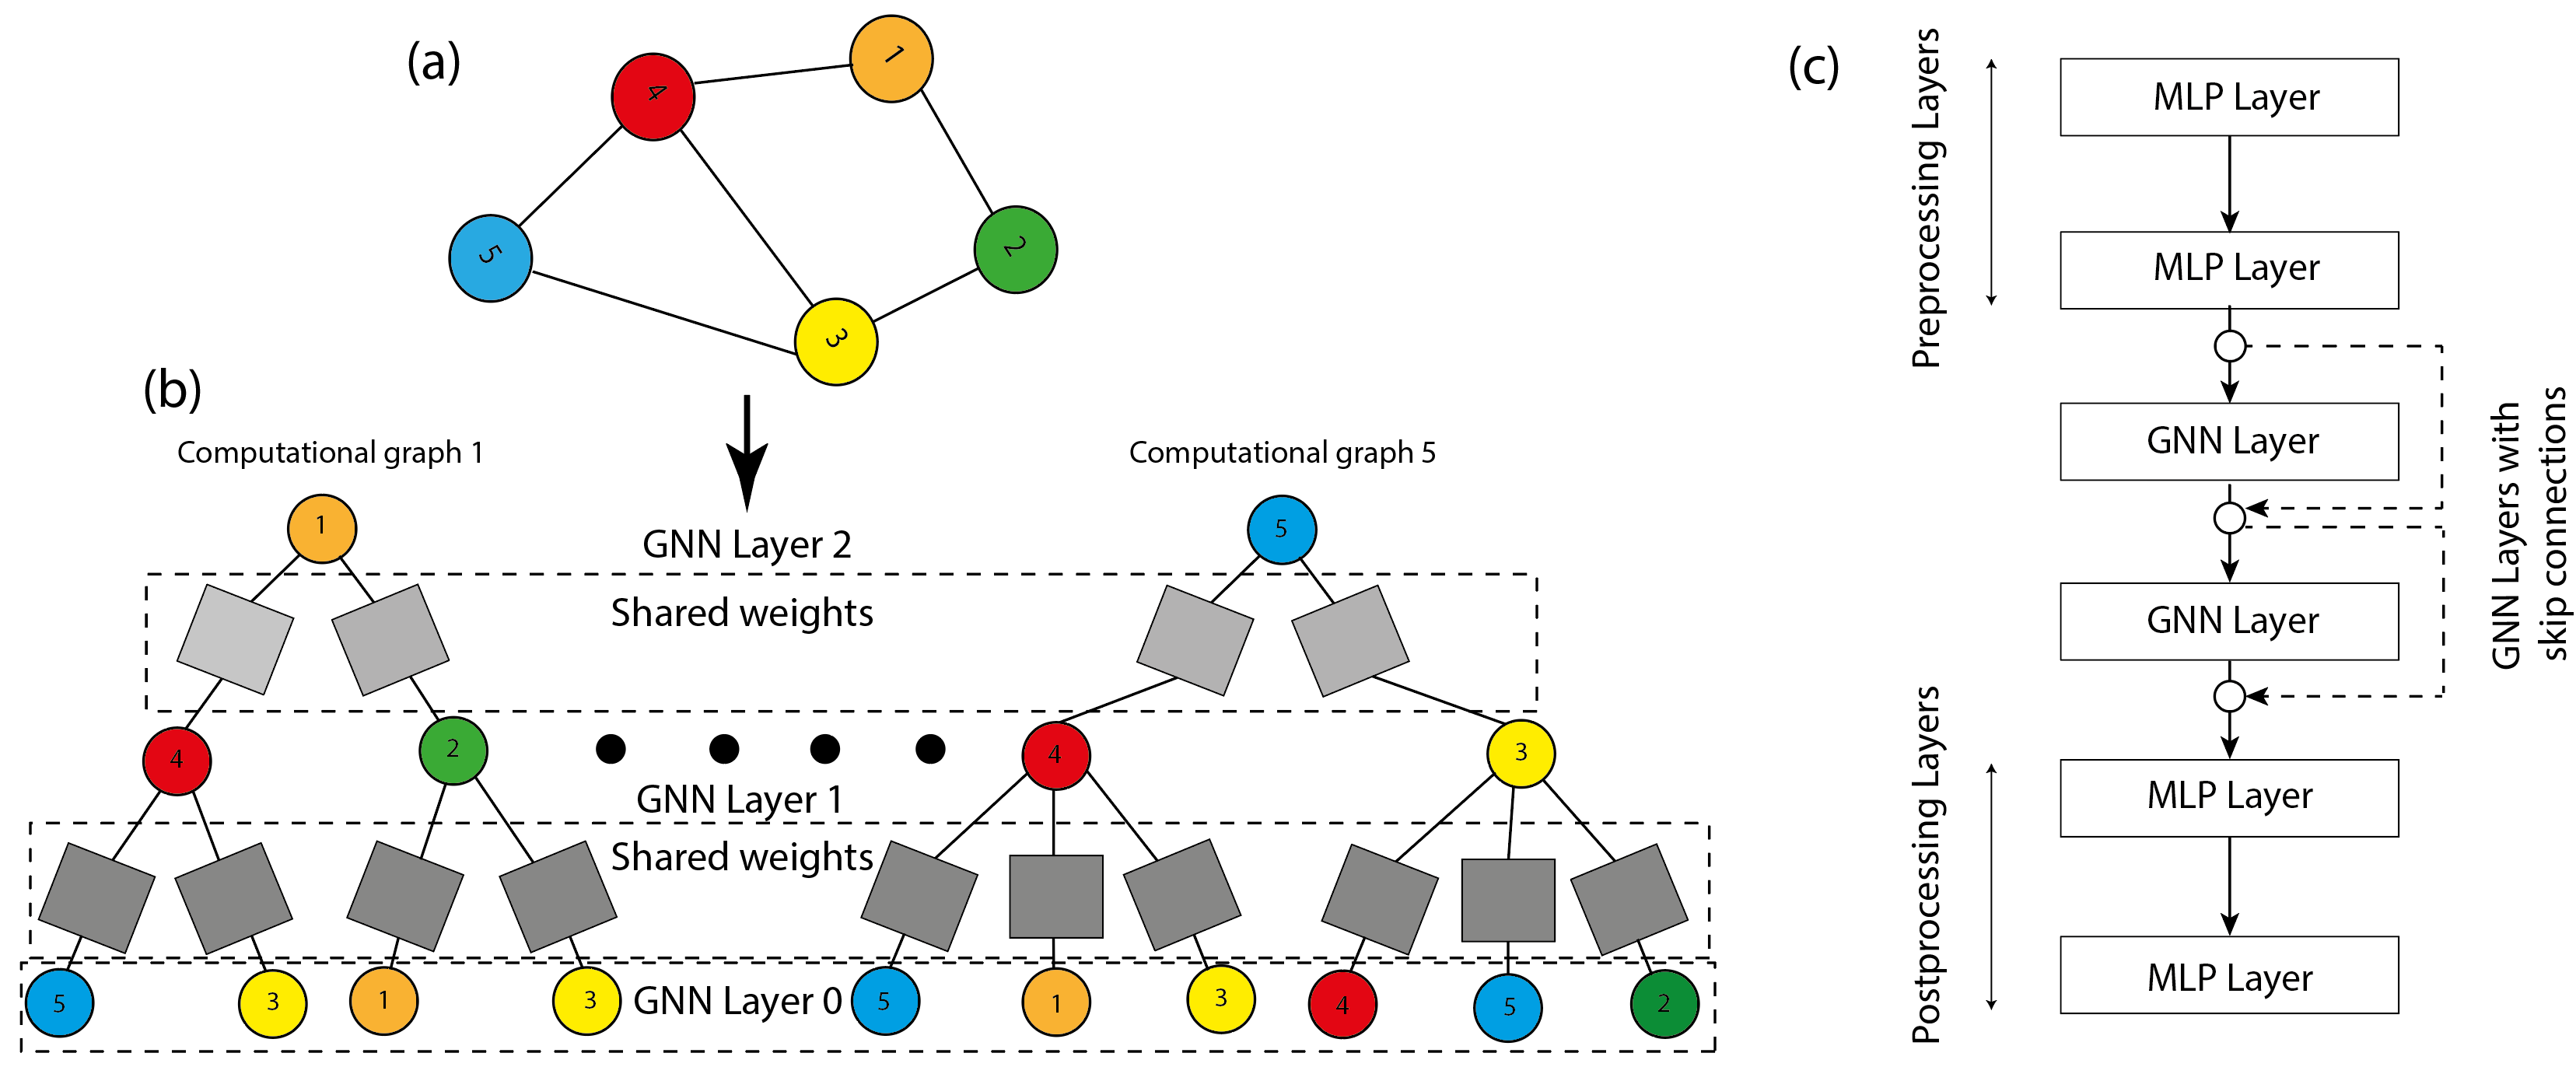
\includegraphics[width=12.6cm]{figures/GNNs_2.png}
    \caption{Convolutional GNN (a) Example of graph structure (b) For each node computational graph is constructed, where each layer contains aggregation functions with shared waits across that layer (c) Upscaled vision of CGNN.}
    \label{fig:gnn}
\end{figure}

GNNs have been successful in many applications \cite{zhou2020graph}.  Recently, GNNs have found application in materials science, showing promise in tasks such as crystal structure prediction and property prediction.

In the context of crystal structure prediction, GNNs can be used to model the interactions between atoms in a crystal lattice and predict the resulting arrangement of atoms. This approach has proven highly effective, with some studies reporting accuracy comparable to the traditional ab initio computational methods, such as density functional theory (DFT) calculations \cite{xie2018crystal, li2023graph}.

\begin{figure}[H]
    \noindent
    \centering
    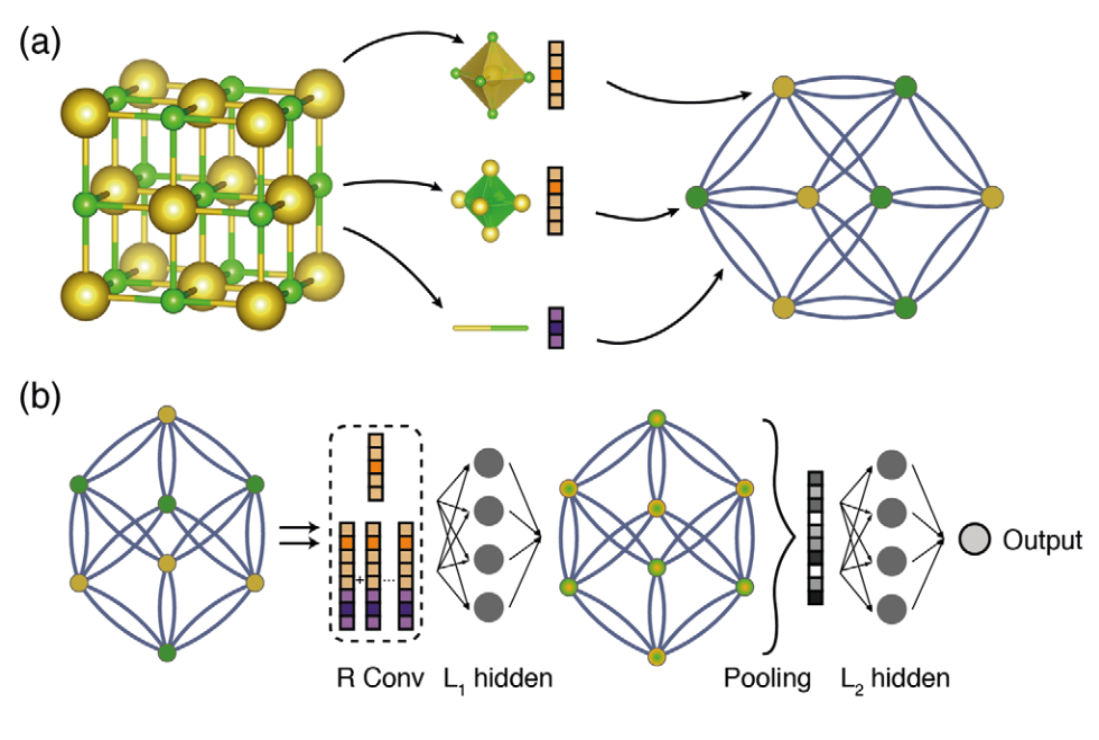
\includegraphics[width=10.6cm]{figures/CGCNN.png}
    \caption{CGNN. Illustration of the crystal graph convolutional neural networks. (a) Construction of the crystal graph. Crystals are converted to graphs with nodes representing atoms in the unit cell and edges representing atom connections. Nodes and edges are characterized by vectors corresponding to the atoms and bonds in the crystal, respectively. (b) Structure of the convolutional neural network on top of the crystal graph. R convolutional layers and $L_1$ hidden layers are built on top of each node, resulting in a new graph with each node representing the local environment of each atom. After pooling, a vector representing the entire crystal is connected to $L_2$ hidden layers, followed by the output layer to provide the prediction. Taken from \cite{xie2018crystal}}
    \label{fig:cgnn}
\end{figure}

One of the key advantages of GNNs for materials science applications is their ability to handle large and complex graph structures, which is often the case for crystal structures. Additionally, GNNs can be trained on large datasets, allowing them to capture complex patterns in the data that are not easily modeled using traditional methods.

As a result, GNNs have been actively researched in the field of materials science in recent years, with a growing body of literature demonstrating their effectiveness for a variety of tasks. In one of the earliest works that used GNNs for crystal properties prediction, \cite{xie2018crystal}, the authors use Graph Convolutional Neural Network with the representation of the elementary cell of the crystal in the form of a graph, taking into account periodicity. The information about atoms is stored in the graph nodes, while graph edges represent interatomic distances.

% (Nikita) Either we should do a proper explanation of differnt kinds of GNNs,
% or drop it alltogether. Truisms like "message passing is when messages are passed"
% is unhelpfull

% Message-passing graph neural networks (MP-GNNs) are a class of GNNs that operate by iteratively exchanging information or ``messages" between nodes in a graph.
% (Nikita) This is also true for CGNN
% The goal of this message-passing process is to allow each node to aggregate information from its neighbouring nodes in order to make a prediction.


%Figure example for that section \cite{xie2018crystal, choudhary2021atomistic, chen2019graph, park2020developing}


The next significant advancement in this field involved the application of methods based on a more advanced variant of GNN, known as the message-passing neural network. MatErials Graph Network (MEGNet) \cite{chen2019graph} is designed to address the limitations of existing machine learning models. It incorporates global state attributes and allows for composability.  The MEGNet models outperform prior machine learning models in predicting properties such as internal energy, enthalpy, Gibbs free energy, formation energies, band gaps, and elastic moduli. MEGNet also presents two strategies to address data limitations in materials science and chemistry. These strategies include a physically-intuitive approach to unify multiple free energy MEGNet models into a single model and using transfer learning from a larger data set to improve property models with smaller amounts of data. 

\begin{figure}[H]
    \noindent
    \centering
    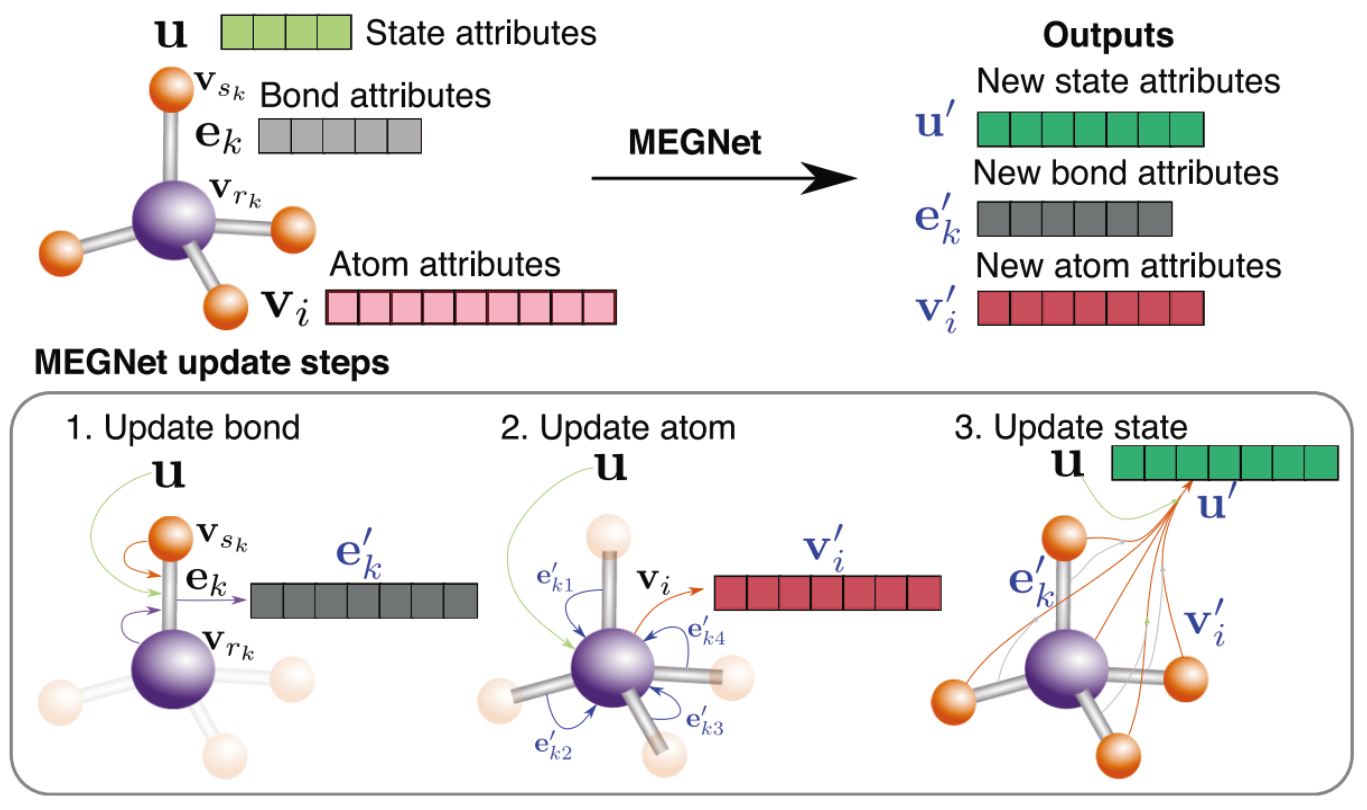
\includegraphics[width=10.6cm]{figures/megnet.png}
    \caption{An overview of a MEGNet module. The initial graph is represented by the set of atomic attributes $V=v_i$, bond attributes $E =\{(e_k, r_k, s_k)\}$, and global state attributes $u$. In the first update step, the bond attributes are updated. Information flows from atoms that form the bond, the state attributes, and the previous bond attribute to the new bond attributes. Similarly, the second and third steps update the atomic and global state attributes, respectively, by information flow among all three attributes. The final result is a new graph representation. Taken from \cite{chen2019graph}.}
    \label{fig:megnet}
\end{figure}

However, constructing the edges of the structure graph based on the atoms pairwise distances fails to account for the directional information between atoms. To address this issue, Gasteiger et al. \cite{gasteigerDirectionalMessagePassing2022} developed a graph neural network model that embeds directional information in the form of message transformations based on the angle between two atoms. The transformed messages are then propagated using the message-passing mechanism. Notably, the embeddings of the directional messages are rotational equivariant. DimeNet \cite{gasteigerDirectionalMessagePassing2022} utilizes the spherical Bessel function and spherical harmonics to construct an orthogonal representation of directional messages. This approach achieves better performance with fewer parameters (75\% reduction) compared to the standard Gaussian radial basis representation used by SchNet.

DimeNet++ \cite{gasteigerFastUncertaintyAwareDirectional2022} is an improved version of DimeNet that addresses the issue of combinatorial representation explosion by reducing the number of embeddings in the directional message passing block.
In the original DimeNet, every message between interacting pairs is embedded separately, resulting in a combinatorial explosion of embeddings. The situation becomes worse in the interaction block, where every triplet is embedded to represent the bond angles. This makes operations in the directional message passing block 15x more expensive than elsewhere in the model. To address this issue, DimeNet++ replaces the bilinear layer used in the original directional message passing block with a simple Hadamard product and compensates for the loss in expressiveness by adding multilayer perceptrons (MLPs) for the basis representations. This results in the same accuracy as the original DimeNet, at a fraction of the computational cost.
DimeNet++ also leverages the fact that certain parts of the model use a higher number of embeddings by reducing the embedding size in these parts via down- and up-projection layers. This both accelerates the model and removes information bottlenecks.
In addition to these improvements, the authors found that using four layers performs similarly to the original six for some energy prediction tasks. They also observed that larger batch sizes significantly slowed down convergence, and mixed precision caused the model precision to break down completely. However, the relative error of DimeNet is below float16's machine precision, which, indeed, can be expected.

GATGNN \cite{louis2020graph} is another variant of GNNs based on the attention mechanism. It introduces a model based on graph neural networks composed of multiple graph-attention layers and a global attention layer to predict inorganic material properties. The model learns the complex bonds shared among the atoms within each atom's local neighborhood, and the global attention layer provides the weight coefficients of each atom, improving the model's performance. This approach allows the model to capture the different contributions of the atoms in the crystal to the global material property. The paper highlights the limitations of existing structural descriptors and the characteristics of desired structural descriptors. It discusses the use of graph neural networks in material property prediction and introduces the attention mechanism to learn the contribution of different context vector components to the merged context vector.

GemNet~\cite{gasteiger2021gemnet} is an improved architecture that is based on DimeNet++.
%  The model was developed on the COLL dataset, but it has been demonstrated to be generalizable to other datasets such as MD17 without requiring any changes to its architecture. 
The architecture of GemNet incorporates three different forms of interaction: geometric message passing, one-hop geometric message passing, and pure atom self-interaction based on atom embeddings. Ablation studies have shown that all three interaction forms benefit the model's performance.
While two-hop message passing introduces significant computational overhead, it is mitigated by a down-projection layer and by the ablated GemNet-T model. Interestingly, the GemNet-T model performs remarkably well on the MD17 dataset, but not on COLL. The author suggests that one-hop message passing is expressive enough for certain practical use cases. In contrast, two-hop message passing provides an advantage for more challenging tasks that involve fitting multiple molecules at once.
In typical machine learning models, the variance of activations is stabilized using normalization methods, which have been shown to have various positive effects on training. However, these methods can have undesirable side effects in the context of molecular regression. To address these issues, GemNet stabilizes its variance by introducing constant scaling factors, as suggested by Brock et al. \cite{brockCharacterizingSignalPropagation2021}. Skip connections, non-linearities, message aggregation, and Hadamard/bilinear layers primarily impact the activation variance. Simple empirical scaling factors are sufficient to keep the activation variance roughly constant. Other measures, such as adaptive gradient clipping, scaled weight standardization, or weighting the residual block with zero at initialization, turn out to be not very beneficial for the accuracy of the model.
In summary, GNNs have gained widespread popularity in the field of material property prediction. They naturally provide desirable inductive bias by respecting symmetries and interaction locality and demonstrate state-of-the-art performance. Being deep learning methods with a large number of parameters, they benefit greatly from the increased amounts of data.

\subsection{Material design}
\label{sec:inverse}
\subsubsection{High-throughput screening}
\label{subsec:High-throughput}
\begin{figure}[H]
	\noindent
	\centering
	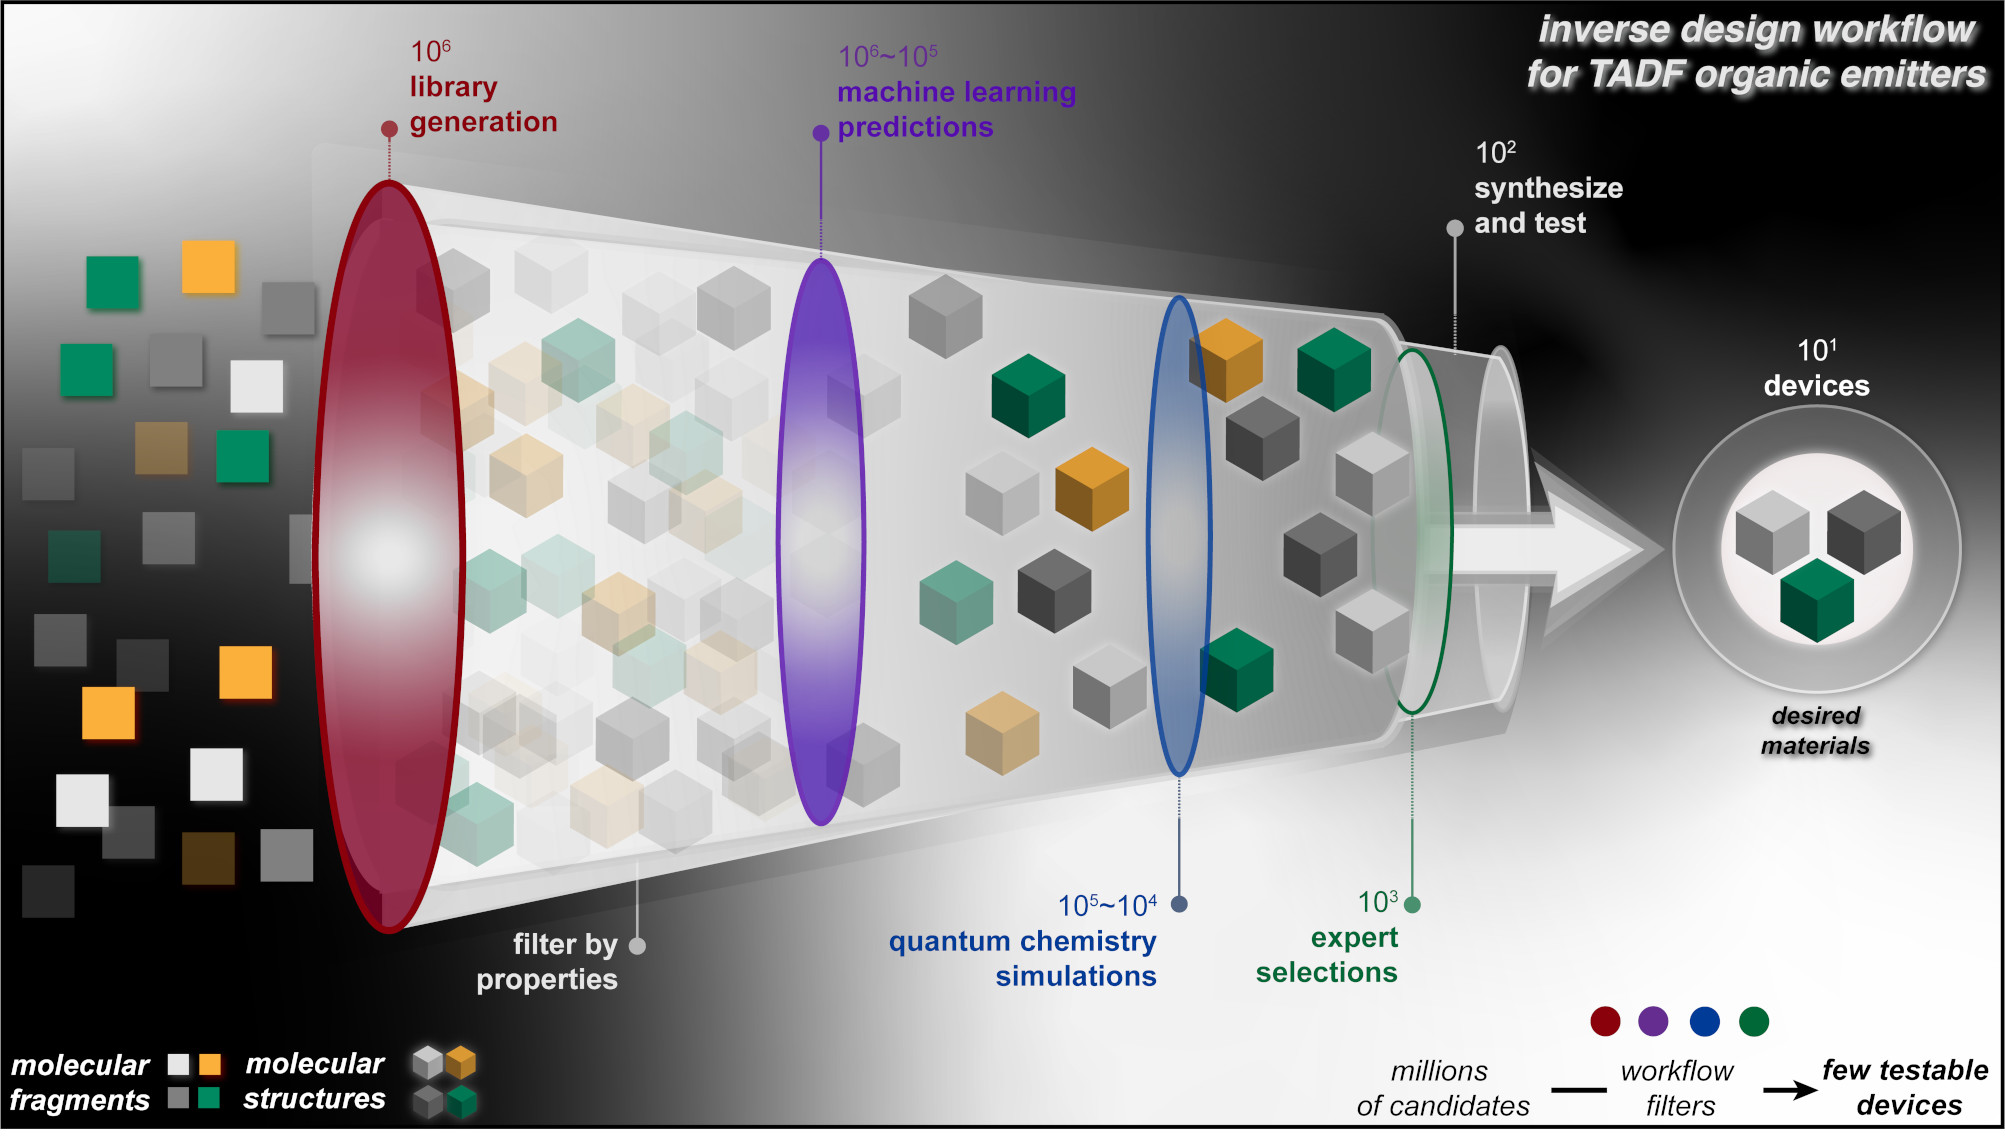
\includegraphics[width=\textwidth]{figures/hts.jpeg}
	\caption{HTS for screening thermally activated delayed fluorescence organic emitters, starting from selecting fragments to the device integration. Taken from ~\cite{pollice2021data}.}
\label{fig:HTS}
\end{figure}

High-throughput screening (HTS) can be viewed as the most straightforward computational material design technique. It consists of an expert-provided algorithm for generating candidate materials and a computational module that predicts the target properties of a material. It can work either ab-initio or using machine learning. The success of HTS depends on the quality of the initial screening scope, which experts in the field should carefully define. To reduce the cost of HTS, computational funnels may be used, in which cheaper or easier-to-compute properties are used as initial filters, with more sophisticated methods or properties used to narrow down the pool of candidates for final selection. An example HTS pipeline is presented in figure~\ref{fig:HTS}.

HTS has been successful in identifying a variety of materials~\cite{song2021usability,li2018high,sarikurt2020high}. Zhang et al. \cite{zhangHighthroughputComputationalScreening2019} review the use of high-throughput computational screening and data mining to discover 2D materials.

In another study \cite{zhang2018effective}, the authors present several examples of the use of computational screening to identify promising 2D materials for various applications. They use DFT calculations to screen a dataset of over 150 \ce{Na}-based layered materials, identifying potential sodium-based battery electrodes with desirable properties such as high average voltage, high sodium ion mobility, and low volume change during the intercalation/de-intercalation of \ce{Na} ions. In addition, the authors show the use of high-throughput screening to identify 2D photocatalysts with positive phonon dispersions, indicating that they may be experimentally exfoliated.

First-principles calculations combined with high-throughput screening are used to identify quantum spin Hall insulators, materials with a specific type of topological order that could be used in spintronic devices \cite{mounet2018two,Olsen2016Designing, Padilha2016new, Xu2013Large, Yu2017Strain, Zhang2017Correction}.


Machine learning methods have played an important role in identifying layered, exfoliatable materials. Exfoliation techniques,  such as mechanical cleavage, surfactant-assisted ultrasonication, and ion intercalation, remain a popular way to prepare various 2D materials. These techniques have played a significant role in the exfoliation of 2D materials from their corresponding layered bulk materials, such as graphene, TMDs, MXenes, and phosphorene \cite{novoselovElectricFieldEffect2004, nicolosiLiquidExfoliationLayered2013,colemanTwodimensionalNanosheetsProduced2011,liBlackPhosphorusFieldeffect2014,mounetTwodimensionalMaterialsHighthroughput2018,naguib25thAnniversaryArticle2014}. Therefore, finding materials that can be exfoliated is an important task.

Nicolas Mounet et al. in \cite{mounet2018two} performed high-throughput calculations using van der Waals density functional theory to predict easy exfoliating 2D materials. More than 100,000 unique crystal structures were extracted from public databases for selection using a specially designed protocol. As a result, more than 5000 structures were filtered and classified as layered structures. In the second stage, selected structures were validated with DFT computations. The result of the study is 1,036 candidate materials for easy exfoliation.

% (Nikita) just another study...
% In material design, one example of the successful application of machine learning is the work by Ma et al. \cite{ma2021large}, in which they used a number of machine learning methods as high-throughput screening (HTS) in combination with ab initio calculations. The authors reported the discovery of 60 novel stable 2D ferroelectric materials.

HTS search performance is limited by the candidate evaluation speed, and machine learning offers an obvious way. The paper by Juhwan Noh et al.~\cite{nohUncertaintyQuantifiedHybridMachine2020} is a typical example of this work. They combine DFT, machine learning (ML), and HTS. The authors use pre-trained machine learning to do the initial screening, followed by DFT, for more precise estimation. The authors built on the crystal convolutional neural network (CGCNN) \cite{parkDevelopingImprovedCrystal2020} model, which we discuss in subsection~\ref{subsubsec:gnns}. They modified it in two ways. First, they use the hyperbolic tangent instead of softplus as the activation function, which regularizes the latent vector within the range of $(-1, 1)$. This causes crystal feature vectors with similar properties to be clustered in the latent space. Secondly, they use Monte Carlo dropout \cite{galDropoutBayesianApproximation2016} to quantify the uncertainty of the predictions. It generates multiple slightly different copies of the model by randomly dropping some connections between neurons. The diversity among the predictions of the model copies is treated as an uncertainty estimate.

In a recent article \cite{merchant2023scaling}, a combined approach using various methods for generating new crystalline structures was also proposed, along with a vast number of DFT calculations to determine their properties. The article suggests and implements scaling the initial dataset for material research through active learning. For this purpose, a pipeline was proposed for generating crystalline lattices of various structures and compositions, unlike those presented in the initial dataset. The generated candidate structures are filtered by a GNN and further calculated using DFT. This iterative method of enriching the database was proposed to yield hundreds of thousands of stable structures. Some were selected as targets for synthesis in an automated laboratory and were obtained experimentally \cite{szymanski2023autonomous}.
% Nikita: nice, but no ML or 2D materials
% A method introduced by Philipp Wollmann et al. in \cite{wollmannHighthroughputScreeningSpeeding2011}, developed for the rapid and accurate screening of porosity in materials. This tool is capable of identifying high surface area materials in a short time, with the authors demonstrating its use in less than 5 minutes for a set of 12 samples. The tool has been applied to a variety of materials, including zeolites, metal-organic frameworks (MOFs), and covalent materials, which have all achieved new records in terms of porosity and gas capture ability. The Infrasorb-12 system is based on the optical detection of adsorption heat and has been shown to have good applicability to reference materials. It has been successfully used in the discovery of new porous MOFs consisting of cobalt and the BTB (benzene-1,3,5-tribenzoate) linker. The Infrasorb-12 system is developed to facilitate the discovery of new porous materials and broaden the range of materials suitable for applications in gas storage, selective adsorption, catalysis, and life science.

% Geoffroy Hautier in his paper \cite{hautierFindingNeedleHaystack2019}, presents examples of HTS computational screening, including the search for transparent conducting materials (TCMs) and materials with large direct band gaps \cite{varleyElectronicStructureDefect2014,bhatiaHighMobilityBismuthbasedTransparent2016}. DFT calculations was used to screen a dataset of over 6000 oxides, identifying a small number of materials with low hole effective masses and potential for p-type dopability, including \ce{PbMO3} \ce{(M=Ti, Hf, Zr)}, \ce{B6O}, and \ce{Ba2BiTaO6}. In the search for materials with large direct band gaps, the authors used a similar approach to screen a dataset of non-oxides, specifically phosphides, and identified boron phosphide (\ce{BP}) as a promising p-type TCM \cite{varleyHighThroughputDesignNonoxide2017}. Joel B. Varley et al. also discuss the importance of considering defects in material screening, as defects can significantly impact the properties of materials. In addition, they discuss the use of machine learning techniques to predict materials properties, which could further accelerate the materials discovery process.

Overall, high-throughput computational screening accelerated by machine learning and data mining offers a powerful tool for discovering novel 2D materials, and the research community expects that these methods will continue to play a significant role in the development of materials science. By using materials databases and computational methods based on advancements in machine learning, researchers can efficiently gather, access, store, and analyze materials data, facilitating the design of materials with specific properties and applications. These methods have already led to the discovery of several promising 2D materials with potential applications in areas such as energy storage and electronics, and they have the potential to identify other functional 2D materials, such as 2D superconductors, photocatalysts, and photoelectronic materials.

\subsubsection{Evolutionary and global optimization}
\label{subsec:Evolutionary}
Evolutionary methods are a class of metaheuristic algorithms that are used for solving complex optimization problems that involve a large number of variables and constraints. Biological evolution processes, swarm behavior, and physical laws inspire these algorithms. Evolutionary methods are broadly classified into two categories: single-solution based and population-based metaheuristic algorithms; see figure \ref{fig:metaheuristics} for details. Single-solution based metaheuristics use a single candidate solution and improve it using local search, but they may get stuck in local optima. Population-based metaheuristics use multiple candidate solutions to maintain diversity in the population and avoid getting stuck in local optima \cite{katochReviewGeneticAlgorithm2021}. Those methods avoid local minima at the cost of computing multiple evolution processes at once.

\textbf{Genetic algorithm (GA)} is one of the most widely used evolutionary methods miming the Darwin theory of survival of the fittest in nature~\cite{darwin1859}. The basic elements of GA include encoding the problem at hand in some representation, usually a bit-vector, fitness selection function, and biological-inspired operators such as selection, mutation, and crossover.

The principle of genetic algorithms is to start with a population of potential solutions representing a set of possible solutions to the optimization problem. Each solution is evaluated based on a fitness function that measures how well it solves the problem. The solutions with higher fitness are more likely to be selected for reproduction.

Reproduction involves selecting two solutions from the population and creating a new solution (offspring) by combining parts of the two parents. This process is called crossover. The offspring may also undergo random mutations, where a small portion of the solution is changed randomly. The idea behind mutation is to introduce new solutions into the population that may not have been explored before, analogous to local search.

The refreshed population, comprising parents and offspring, undergoes the same selection cycle, crossover, and mutation. This iterative process is repeated for several generations, typically until a stopping criterion is met, such as a maximum number of generations or a minimum acceptable fitness value.

Over successive generations, the population gradually converges toward superior solutions, driven by the selection process that favors solutions with higher fitness scores. The genetic operators of crossover and mutation introduce diversity into the population, which helps avoid getting stuck in local optima.

\begin{figure}[H]
    \centering
    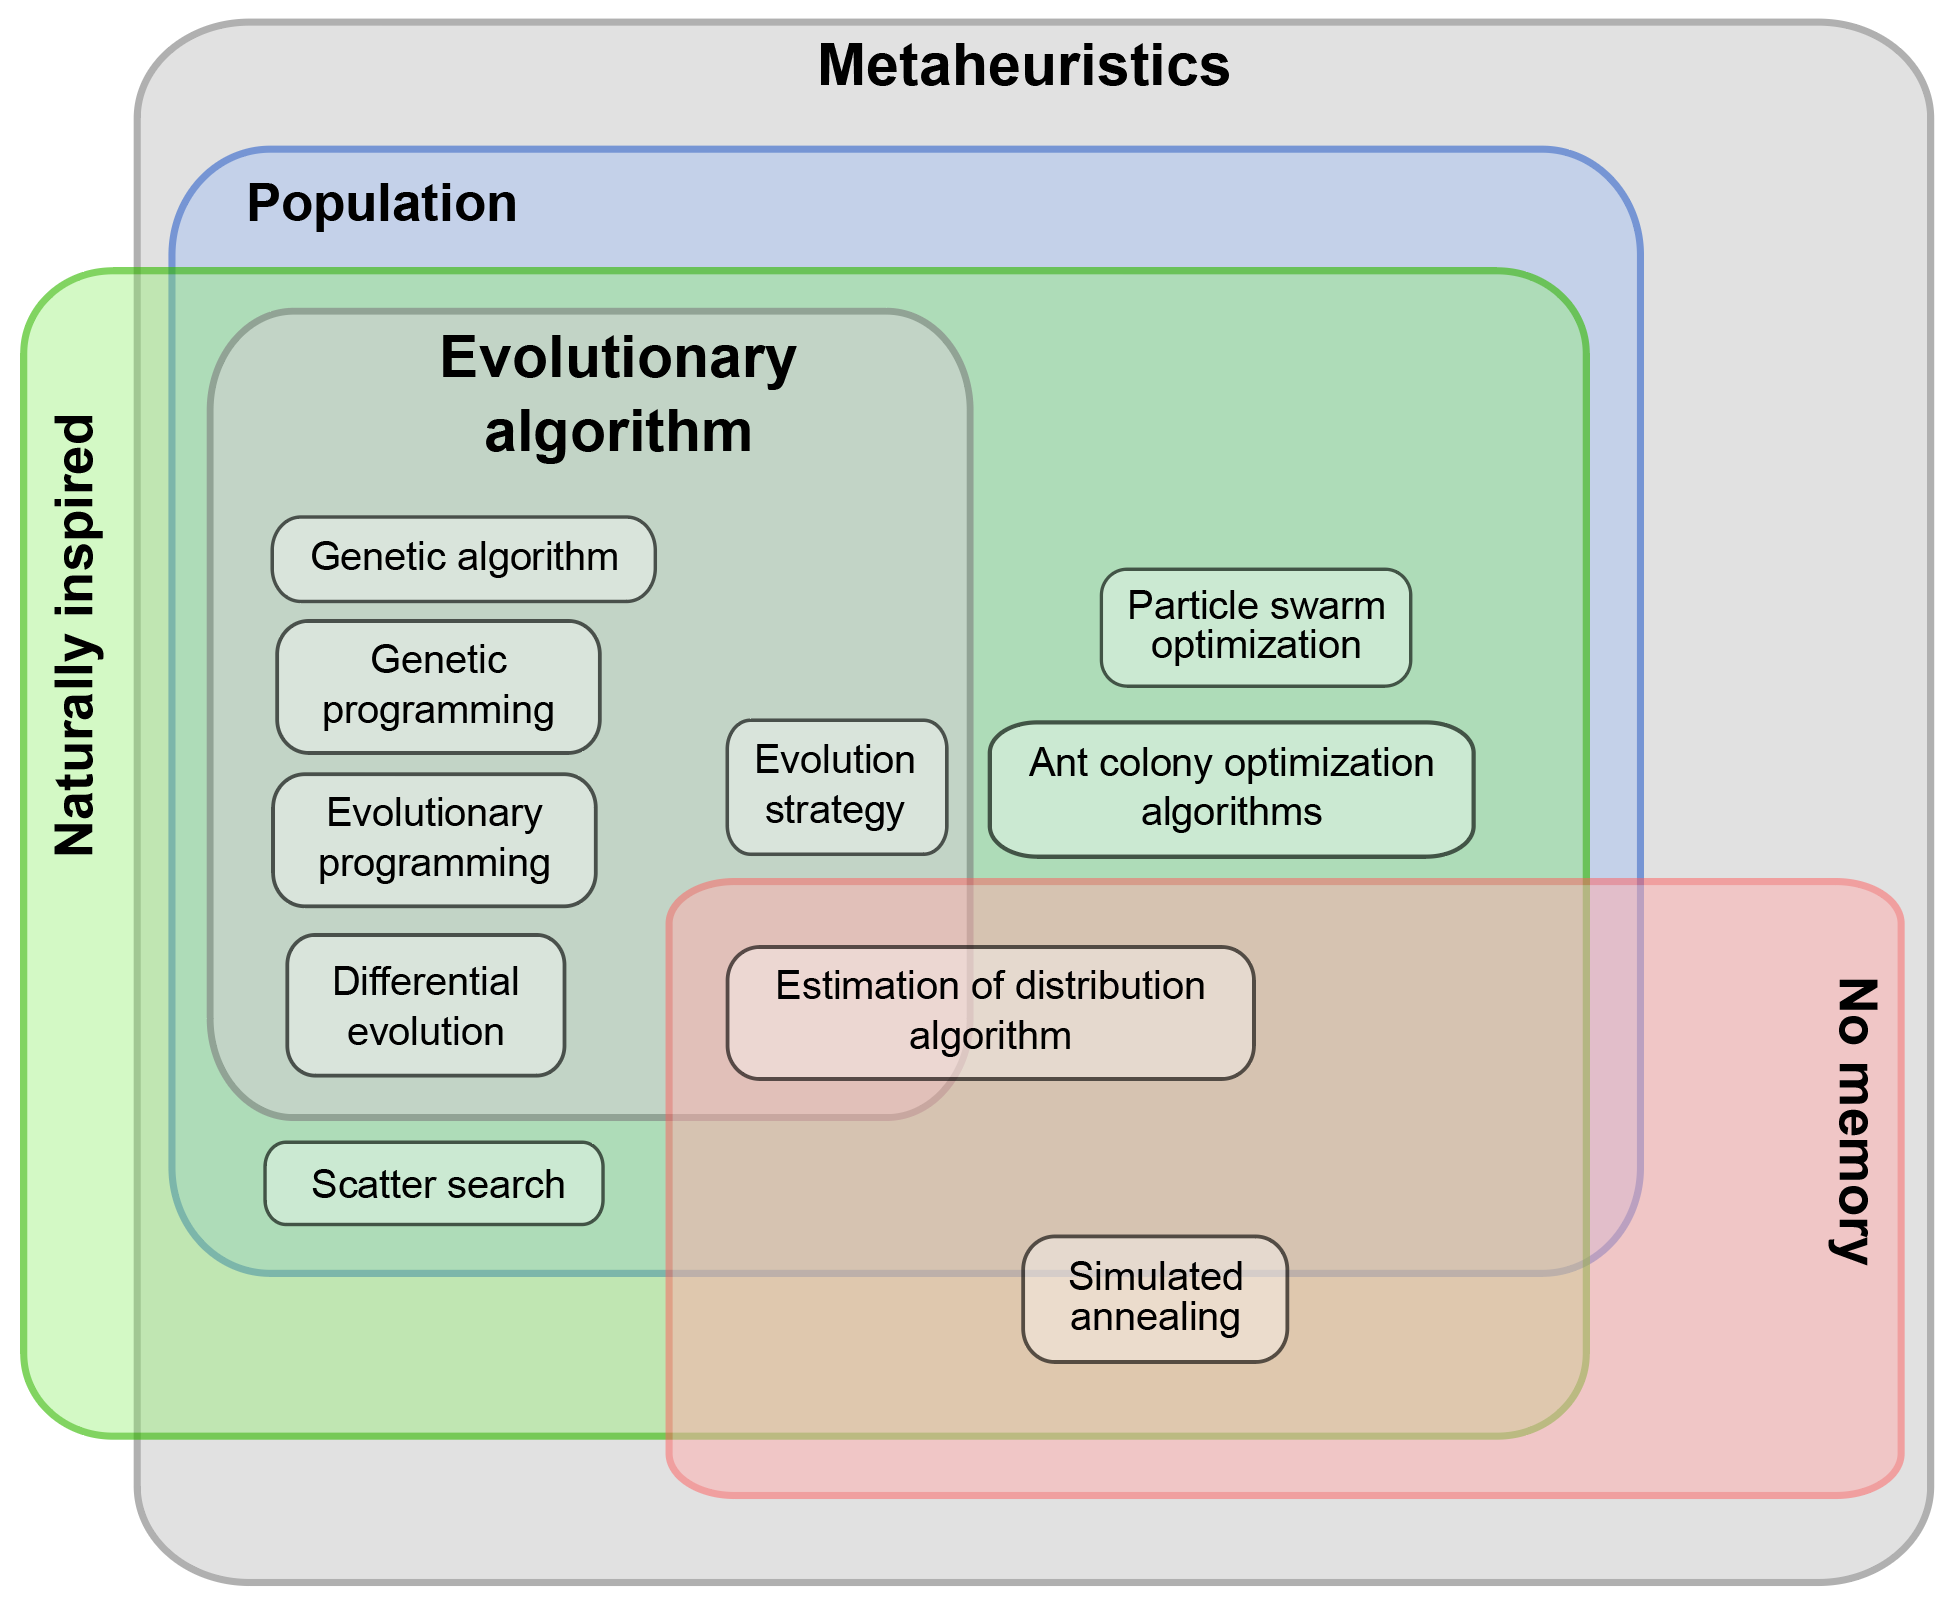
\includegraphics[width=\textwidth]{figures/Metaheuristics.png}
    \caption{Classification of metaheuristics algorithms. Adapted from ~\cite{metaheuristics}
    }
    \label{fig:metaheuristics}
\end{figure}

The success of genetic algorithms is due to their ability to explore a large search space efficiently and find good solutions even in the presence of noise, uncertainty, and the lack of gradient information.

Evolutionary algorithms have a rich history of being used for inverse design~\cite{johnson1994genetic, sloss20202019}. In the rest of the section, we review notable cases of their application for designing 2D systems.

In \cite{hakanssonInverseDesignedPhotonic2005} Andreas H{\aa}kansson and Jose Sanchez-Dehes present a method for the inverse design of photonic crystals (PhCs) \cite{PhotonicCrystals2008,johnStrongLocalizationPhotons1987} using a GA. PhCs are materials with unique properties that can be used to design optical devices with sub-wavelength cavities and low loss. These materials have potential applications in various fields, including telecommunications, sensors, and energy harvesting \cite{Gan2015Photonic, Rifqi2019Modelling, Zhao2014Spherical}. While traditional design methods rely on physical intuition and insight into PhCs nature. In contrast,  the inverse design enables the optimization of functional devices based on predefined constraints. This approach has been used to design a variety of PhC components, including spot-size converters \cite{spuhler1998evolutionary}, photonic band-gap materials \cite{shen2003design}, cavities for QED experiments \cite{geremia2002inverse}, low loss PhC waveguide bends \cite{haakansson2005high}.

In particular, the work \cite{haakansson2005inverse} considers the design of a de-multiplex waveguide coupler (DEMUXWGC). The purpose of the device is to separate and couple two wavelengths from a single dielectric waveguide (WG) to two separate PhC-WGs. The design variables for the DEMUXWGC are the coupling efficiency and crosstalk attenuation for each channel and wavelength. To estimate these parameters, the authors calculate the amplitudes of the electric field in the center of the PhC waveguides. Since the PhC-WG is designed to support a single mode, the total intensity flux of the coupled mode can be scaled proportionally with the maximal amplitude of the mode profile.

Kildishev et al.~\cite{kildishevStochasticOptimizationLowloss2007a} use evolutionary methods to design a three-layer near-field lens (NFL), a lens designed to operate on a scale much smaller than the wavelength of light. The authors use three optimization methods: simulated annealing (SA), which is based on the physical analogy of cooling crystal structures; a genetic algorithm; and particle swarm optimization. SA had the best result.

The authors also note that the practical fabrication of optimal devices requires taking additional considerations into account, such as geometrical limitations, material properties, and the impact of the fabrication process on material properties. These constraints can affect the performance of the materials and must be considered in the design process. Overall, the authors demonstrate the successful use of optimization techniques for the design of metamaterials for nanoscale optical sensing and imaging.

Hashim Hassan and Tyler N. Tallman in \cite{hassanComparisonMetaheuristicAlgorithms2021} present a study on the use of global search algorithms to solve the inverse problem of computing strains from conductivity changes in self-sensing materials \cite{Chung2016Self, Rana2016review,SBack,Swait2012Smart,Thostenson2007Multifunctional,Tian2019state,Vlachakis2020Self}. The authors explore the use of three commonly used metaheuristic global search algorithms, namely simulated annealing (SA) based on \cite{ingberAdaptiveSimulatedAnnealing2000, metropolisEquationStateCalculations1953}, particle swarm optimization (PSO) based on \cite{kennedyParticleSwarmOptimization1995, pedersenGoodParametersParticle2010, mezura-montesConstrainthandlingNatureinspiredNumerical2011} and genetic algorithm (GA) based on the work of \cite{raghavanSpectralAnalysisRlines2008, hassanFailurePredictionSelfsensing2020} to solve the ill-posed, multi-modal inverse problem. The study is motivated by the current limitations in determining the underlying mechanical state of a piezoresistive sensor from electrical measurements.
Based on the experimental loading setup, the authors formulated a boundary value problem (BVP) of a plate consisting of an unknown displacement boundary condition. The BVP was integrated with the finite element method (FEM) to solve for the optimum displacement boundary condition. The SA, PSO, and GA algorithms were used to find the solution to the BVP. The authors chose parameter values for the algorithms based on the observation that the plate did not fail during the experiment and the expected applied displacement to be lower than the failure displacement.
The study results indicate that the three global search algorithms were able to find solutions to the inverse problem of computing strains from conductivity changes. The authors draw a quantitative comparison between the three algorithms regarding the quality of the inversely computed displacements and strains, the variability and accuracy of the displacement solutions, and the computational efficiency regarding the fitness function and runtime.

Yinchang Zhao et al. \cite{zhaoSuperconductivityTwodimensionalBoron2016} employ an evolutionary algorithm USPEX combined with ab initio simulations \cite{oganovCrystalStructurePrediction2006,zhuEvolutionaryMethodPredicting2013, ,glassUSPEXEvolutionaryCrystal2006} to search for structural phases of 2D boron allotropes with the goal of discovering new superconducting phases. The authors use the monolayer, bilayer, and thin multilayer 2D boron structures to study superconductivity and perform searches based on the spacing between layers of multi-walled boron nanotubes. The results of the study reveal five energetically stable structures with high symmetry. The authors find that superconductivity is ubiquitous in these newly found boron structures, with $T_c$ values higher than the liquid-helium temperature. The authors attribute the high $T_c$ values to the presence of multiple vibration modes in the electron-phonon coupling (EPC) mechanism.

Study of \ce{Na_xCl_y} systems at various conditions by USPEX algorithm \cite{zhang2013unexpected} predicted two exotic stable compounds, \ce{Na_3Cl} and \ce{Na_2Cl} were found at normal conditions as 2D phases on a graphene substrate \cite{shi2018two}. There are many other USPEX predictions applied to 2D materials \cite{faraji2021computational, popov2021novel}.

Silvia Bahmann and Jens Kortu in \cite{bahmannEVOEvolutionaryAlgorithm2013} developed an evolution strategy-based algorithm for crystal structure prediction called EVO. The algorithm uses crystal structures as individuals and Gibbs free energy as the fitness function that must be minimized. The authors also employed variable-cell structure relaxation \cite{woodleyStructurePredictionTitania2009}, which provides an efficient local optimization and makes the structures and energies comparable for a global search.

The author's implementation of EVO has been successfully applied to find crystal structures of elements in the 3rd main group, encompassing various space groups and utilizing different multiples of the number of atoms in the conventional cell. The authors also found 2D structures, such as a boron sheet, with structural features not previously considered in the literature. \\

Two-dimensional magnetic materials have attracted significant attention due to their potential applications in spintronics and data storage \cite{tongConceptsFerrovalleyMaterial2016, Liu2020Spintronics,huangLayerdependentFerromagnetismVan2017, gongDiscoveryIntrinsicFerromagnetism2017, bonillaStrongRoomtemperatureFerromagnetism2018, Awan20202, Ahn20202D}. Stimulated by these exciting experimental reports, 56 new magnetically ordered monolayer structures were predicted from high-throughput computation to be exfoliated from known magnetic bulk materials \cite{mounet2018two}.
To search for stable 2D magnetic structures, the authors further developed a new computational scheme based on the ab initio evolutionary algorithm USPEX \cite{oganovCrystalStructurePrediction2006,zhuEvolutionaryMethodPredicting2013, ,glassUSPEXEvolutionaryCrystal2006} combined with the spin-polarized density functional theory (DFT).
The initial structures are randomly produced with assigned layer group symmetry and user-defined thickness.
They are assumed to have either ferromagnetic, anti-ferromagnetic or nonmagnetic (NM) orders.
User inputs determine the ratio of different structures (NM, FM-LS, FM-HS, AFM-LS, AFM-HS, FM-LSHS, and AFM-LSHS).
The authors evaluated the reliability and accuracy of their new method by investigating the 2D \ce{CrI3} system. Through this search, they uncovered many new metastable magnetic structures that had not been previously identified in high-throughput computational screenings. Additionally, these structures did not have any known parent bulk materials in the database, indicating that the search was not biased and offered a more comprehensive sampling of the configuration space. The most stable magnetic structure contained 19 atoms per unit cell and was identified as the \texttt{19-P6/mmm} borophene as a stable striped-AFM semiconductor.

Shujing Chen et al. in \cite{chenConstrainedOptimizationTransition2022} have proposed a genetic algorithm for designing high-performing optical sensors, focusing on the use of transition metal dichalcogenide (TMDC) Bloch surface wave (BSW) technology. This technology offers advantages such as an all-dielectric structure, sharper resonance peaks, and a wider wavelength range. However, previous studies have demonstrated that the sensitivity of BSW sensors is typically lower than that of surface plasmon resonance (SPR) sensors when using the standard Kretschmann prism coupling method. To enhance the sensitivity, the researchers proposed a multi-variable, multi-objective optimization method utilizing an improved genetic algorithm. By optimizing such factors as film thickness, periods of one-dimensional photonic crystal (1DPC), the thickness of the defect layer, and the number of layers of TMDC materials, they were able to increase the sensitivity of the sensor significantly. The highest sensitivity was reached using \ce{MoSe2}, \ce{WSe2}, \ce{MoS2}, or \ce{WS2}, resulting in an improvement of 24.3\%, 24.8\%, 22.7\%, or 24.4\% respectively. This optimized BSW sensor has potential applications in various fields, including food safety, environmental monitoring, and biological analysis.

Ankit Mishra et al. in \cite{mishraMultiobjectiveGeneticTraining2018} propose an approach to training and quantifying quantum molecular dynamics (QMD) simulations. The team introduced a multi-objective genetic algorithm (MOGA)-based approach for the reactive molecular dynamics (RMD) method. The method enables large-scale simulations of chemical events in complex materials involving multimillion atoms. The approach is used to study the high-temperature sulfidation of \ce{MoO3} flakes with \ce{H2S} precursors during the chemical vapor deposition (CVD) synthesis of \ce{MoS2} monolayers. The goal was to train ReaxFF \cite{vanduinReaxFFReactiveForce2001} parameters against QMD simulations by estimating the number of \ce{H}-\ce{S}, \ce{Mo}-\ce{O}, and \ce{Mo}-\ce{S} bonds as a function of time. The results showed that the MOGA-based approach for RMD was able to reproduce the time evolution of key reaction events in the QMD simulations.

Tarak K Patra et al. in \cite{patra2017neural} presents a new strategy of utilizing neural networks combined with genetic algorithms to design soft materials without pre-existing databases efficiently. This strategy involves the selection of new candidates for the genetic algorithm based on an objective function that quantifies their properties in relation to target values. The authors note that this approach enables the genetic algorithm to learn from its history, accelerating the process compared to an evolutionary process alone.

Genetic algorithms have also been combined with molecular dynamics to study defects. For example, later, Tarak K Patra et al., in the paper \cite{patra2018defect}, investigate the extended structure of point defects and their dynamical evolution in transition-metal dichalcogenides. A fundamental understanding of the atomic-scale structure and dynamics of defects in these low-dimensional systems and their role in phase transitions is critical for advances in nanotechnology.

This study combines machine learning methods with molecular dynamics simulations to study how point defects in a 2D monolayer of \ce{MoS2} are organized into extended structures. The authors use high-resolution transmission electron microscopy experiments to validate their findings and show how defects evolve from random point defects to extended line defects, which play a role in driving phase transitions from a semiconducting 2H phase to a metallic 1T phase. Simulations and experiments suggest that the alignment of the extended line defects influences the size and shape of the 1T regions. By introducing them into a \ce{MoS2} layer, the relative proportions of the metallic and semiconducting phases can be systematically controlled.

\subsubsection{Machine intelligence}
\label{subsec:intelligence}
Machine learning works by fitting a heuristic, "intuitive" model for the system under study, on the high level, it is the same for both forward and inverse problems. Designing a new material, is, however, a much more difficult problem than predicting properties. Instead of summarizing the information about a given structure and predicting a number, the algorithm must traverse the intractable space of all possible arrangements of elements and find one that is stable and has different properties.

\subsubsection{Generative modeling}
As we discussed previously, raw atomic structures do not match well with the machine learning mathematical and computational apparatus. Hence, generative methods map the structures into a more suitable representation, learn the probability distribution inside this space, and then map from it to the structures. A common aspect of all the methods developed so far is that this second mapping doesn't fully define the structures, but just provides an initial guess which is then refined using the forward models.

\begin{figure}[h]
    \noindent
    \centering
    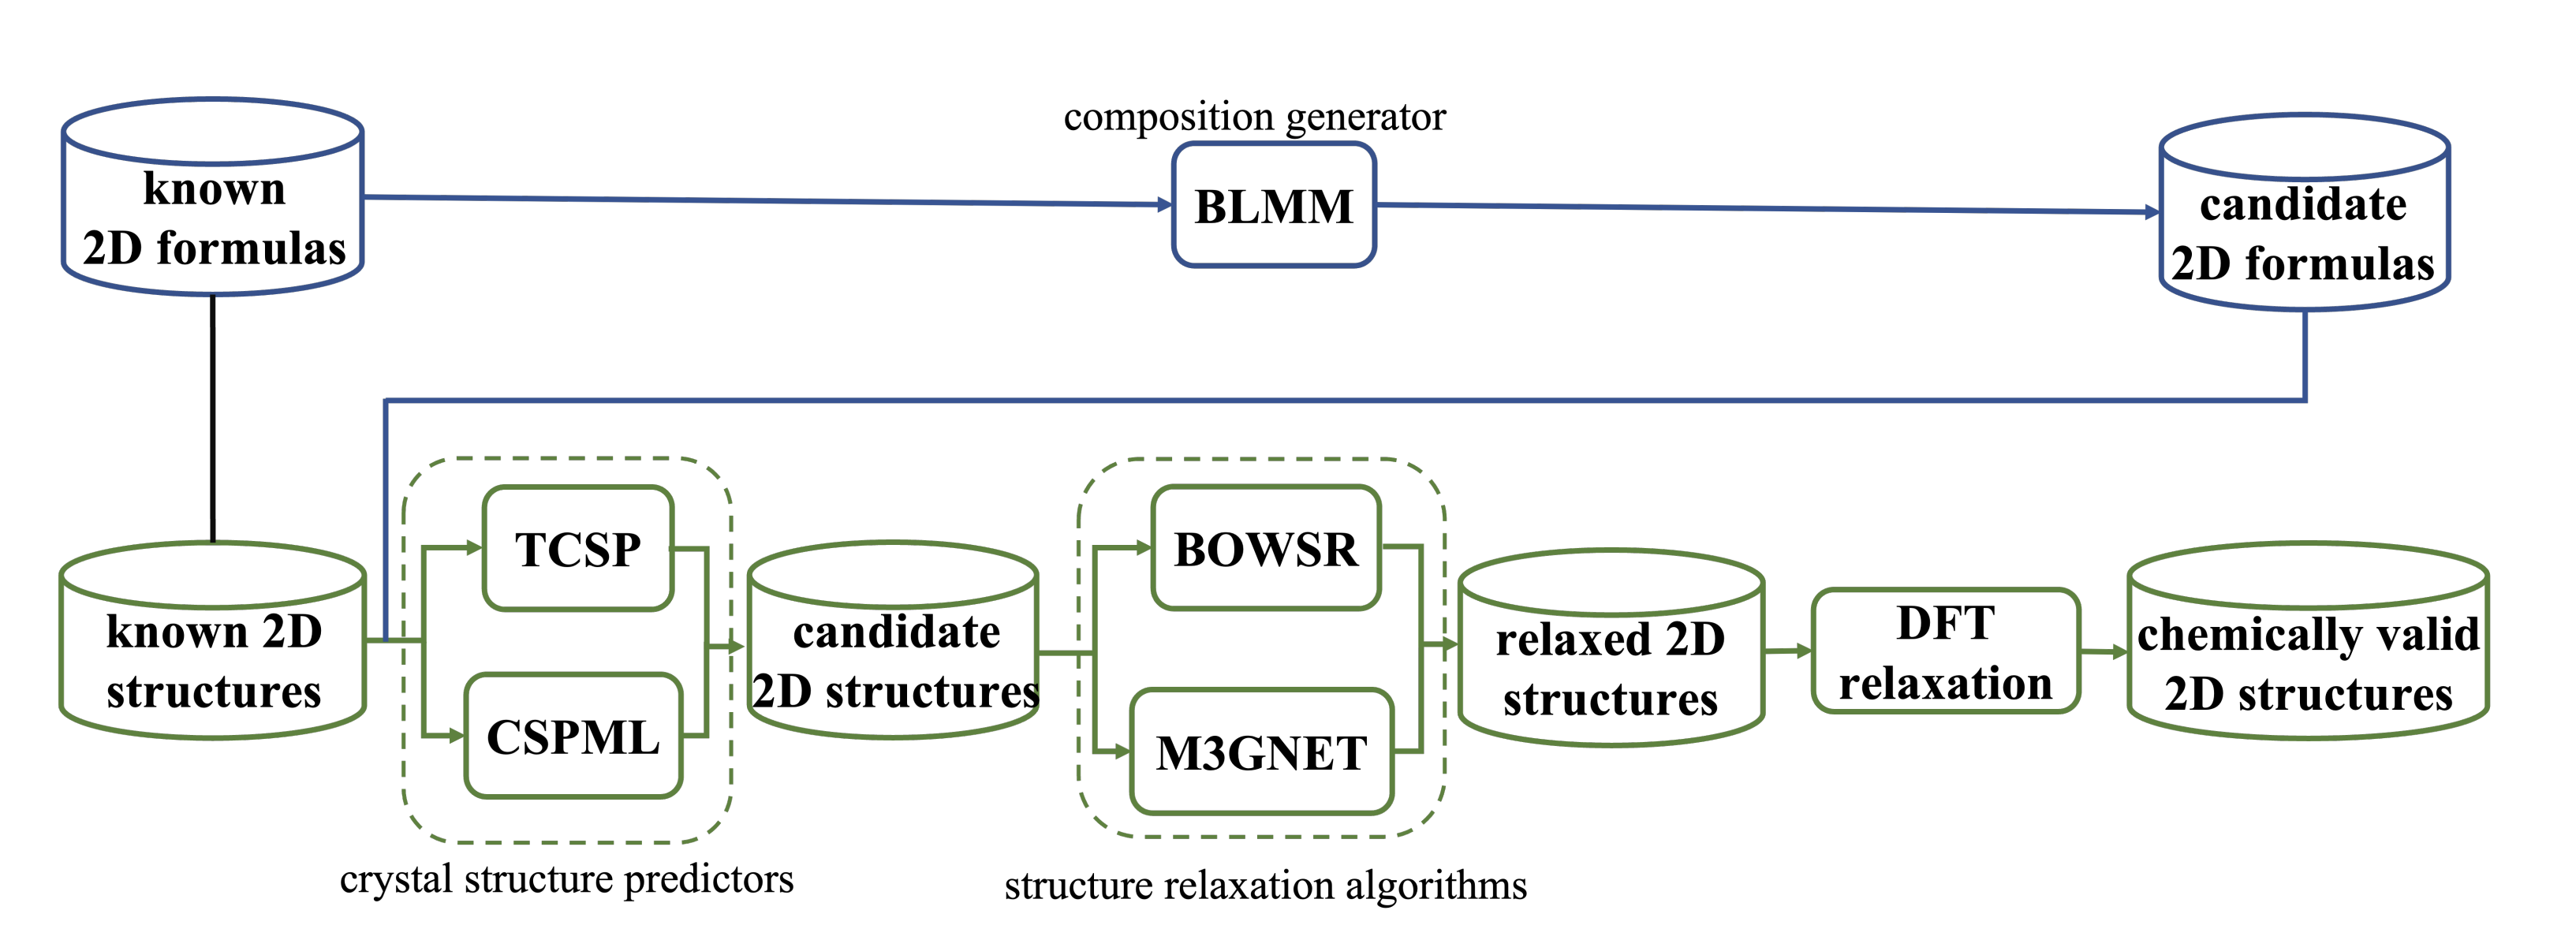
\includegraphics[width=\textwidth]{figures/mat_discovery_pipeline.png}
    \caption{The process for generating 2D materials. It describes the architecture of a material transformer generator (MTG) pipeline. Taken from \cite{dongDiscovery2DMaterials2023}}
    \label{fig:mtg}
\end{figure}
An illustrative approach of this kind is present in figure~\ref{fig:mtg} Rongzhi Dong et al. in \cite{dongDiscovery2DMaterials2023} propose a material transformer generator (MTG), a pipeline for 2D material discovery that integrates a transformer-based 2D material composition generator, two template-based crystal structure predictors, and a graph neural network potential-based structure relaxation algorithm.

Firstly, the material composition is mapped into a sequence and sorted by electronegativities of elements. The distribution over those sequences is learned using Transformer~\cite{vaswani2017attention} in the step called blank language models for materials (BLMM). Notice the information loss.

Secondly, the initial guesses for the structures are produced using two crystal structure prediction algorithms: template-based crystal structure prediction (TCSP)~\cite{wei2022tcsp} and machine learning-based crystal structure prediction (CSPML)~\cite{kusaba2022crystal}. TCSP is based on oxidation state patterns, while CSPML uses a machine learning model to select templates based on structural similarity. For a new 2D formula, both TCSP and CSPML would first select all template structures with the prototype ABC3, but the sorting process differs between the two. TCSP focuses on element distance and calculates the element mover distance score and element oxidation states. On the other hand, CSPML selects candidates solely based on the topological features of the atomic coordinates and does not use any information about the elemental composition.

Thirdly, two machine learning potential-based relaxation algorithms are used to optimize the structures. These algorithms are BOWSR \cite{zuo2021accelerating}, which uses Bayesian optimization with symmetry relaxation and M3GNet \cite{chen2022universal}, which utilizes materials graph neural networks with 3-body interactions as an energy estimation model. 

Finally, the formation energy and e-above-hull energy of structures are calculated using DFT.

A set of known 2D formulas and their structures were collected from open datasets, including C2DB, MC2D, 2DMatPedia, and V2DB. The pipeline was trained using materials from various databases (328,719 formula samples and 12,214 structures).

\textbf{Variational autoencoder (VAE)} is a generative model that consists of two main parts:  encoder and decoder \cite{kingma2013auto} similar to autoencoders (AE) (see figure ~\ref{fig:generative-models} VAE). The VAE core idea is to learn the latent probability space representation of objects presented in a dataset. Sampling vectors from learned latent space and decoding them should give us a new object similar to what is presented in the training dataset.

Juhwan Noh et al. in \cite{noh2019inverse} introduced the first VAE generative model for inverse crystal design. This work proposed a framework to learn continuous material representation in a latent space. The algorithm consists of three steps. Firstly, it represents the material as a 3D image, by diving the space into voxels, and atoms as balls. The second step is training an autoencoder to transform the images into a latent vector. Finally, a VAE is trained to generate new materials in this latent space. The model was trained and tested on a custom \ce{VO} dataset comprising 10981 \ce{V}$_x$\ce{O}$_y$ compounds. The authors reported newly generated metastable VO structures and supported their findings with DFT simulations.

The Crystal Diffusion Variational AutoEncoder (CDVAE) \cite{xie2021crystal} uses a graph neural network to map the materials into a latent vector space. An MLP is used to predict the lattice parameters and chemical composition from a latent vector. Finally, a random unit cell with those parameters is generated and is relaxed using a denoising model. CDVAE has been shown to outperform past methods in tasks such as reconstructing input structures, generating diverse and realistic materials, and creating materials with specific optimized properties.

The latest model that employs diffusion was presented by the Microsoft research team \cite{zeni2023mattergen}. MatterGen is a diffusion model that generates stable, diverse inorganic materials across the periodic table and can be fine-tuned to the generation of materials with a wide properties range. The noise introduction process is designed to independently disrupt the types of atoms, coordinates, and lattice to achieve a physically motivated picture of the randomized material. The equivariant scoring network was pretrained for denoising. The authors claim that, compared to the previous solutions, their model produces materials that are more than twice likely to be new and stable, and also that the model predicts the energy of the material 15 times closer to the local energy minimum.

A variational autoencoder was also trained in \cite{agarwalDataDrivenDiscovery2D2021a}. A conditional type of VAE is used to learn a continuous representation of the materials in a latent space. This research explores the space of 2D materials from the point of view of photocatalysts: these substances can be used for photocatalytic water splitting, a technique to produce hydrogen. This is a task of significant importance since hydrogen as transport fuel promises to alleviate the effects of global warming. 
The authors use a database containing the properties of 2D materials computed via high-throughput density functional theory (DFT) calculations \cite{jainCommentaryMaterialsProject2013}. Based on this data, a generative model learns the representations of 2D materials to generate novel ones sampling from continuous representations. The pipeline to learn the representations of the 2D materials consisted of "cell" and "basis" autoencoders and a segmentation network like in the iMatGen framework. The analysis of the predictions of the "cell" and "basis" encodings was then used to train a conditional VAE, whose latent space was sampled to generate new 2D materials. Subsequently, the novel materials were constrained and narrowed down to qualify as potential catalysts. As a result of passing the $\sim$150 materials through a classification network, 19 materials with a probability of $>0.99$ belong to the stable class. Moreover, it was observed that all 19 shortlisted appeared to be halides since they were the dominant type in the training dataset.


\textbf{Generative adversarial networks (GANs)} represent a class of generative models initially designed to tackle image generation problems as VAEs. GANs are composed of two neural networks, Generator and Discriminator \cite{goodfellow2020generative} (see figure ~\ref{fig:generative-models} GAN). As an input to the generator, it used a Gaussian noise vector, which the generated output discriminator takes as an input to judge if it is a real object or a generated one. During the training, both NNs compete with each other. Thus, generative NN can be trained to generate objects that are hardly distinguishable from those presented in the dataset.

One of the classic examples of generative model usage was presented in \cite{yeung2021global}. The generative model was applied to metasurface properties prediction and metasurface pattern generation. The core of the generative algorithm is a conditional deep convolutional generative adversarial neural network (CGAN).

\cite{kim2020generative} is one of the first examples where conditional GANs were used in tandem with a critic neural network to generate crystals on the base of Mg-Mn-O ternary materials using an image-like representation. They also use a variant of GAN that utilised Wasserstein distance \cite{arjovsky2017wasserstein} between generated material target value distribution and target distribution for additional training stability.

In a recent work by Teng Long et al.  \cite{long2022inverse}, GANs with constraints similar to algorithm architecture as in \cite{kim2020generative} were applied to crystal structure generation. Here, encoding of the lattice constants and atomic positions is done by training the autoencoder to learn latent material representation space, which can be represented as an image. Overall, 50000 structure image representations were generated. However, only 9160 was reasonable because most of the generated structures contained atoms that occupies the same position. 8310 structures among them are distinct. Thus, it was shown that CCDCGAN is capable of reproducing known structures and pushing boundaries by predicting new materials.

In research by Yuqi Song et al.~\cite{song2021computational} GAN with random forest (RF) classifier was proposed as a part of a generative inverse design algorithm to discover new 2D materials. To generate chemically valid compositions at the first stage, GAN learns to generate chemically valid formulas from known datasets. RF classifier trained on a mixed dataset of 2D materials and non-2D used to assign a probability for generated material from the GAN of being 2D material. Here, the probability was used as a ranking criterion, and 1485 hypothetical materials were generated with a probability of more than 0.95. DFT simulations were performed to determine exfoliation energy. As a result, 31 materials were found to have exfoliation energies of less than 200 meV, thus potentially easy to exfoliate. However, the proposed algorithm has its weaknesses; as the authors mentioned, the crystal structure prediction is a weak place here since it uses template-based structure prediction. To generate novel material with a unique structure, a more powerful structure prediction algorithm is needed.

\begin{figure}[H]
	\noindent
	\centering
	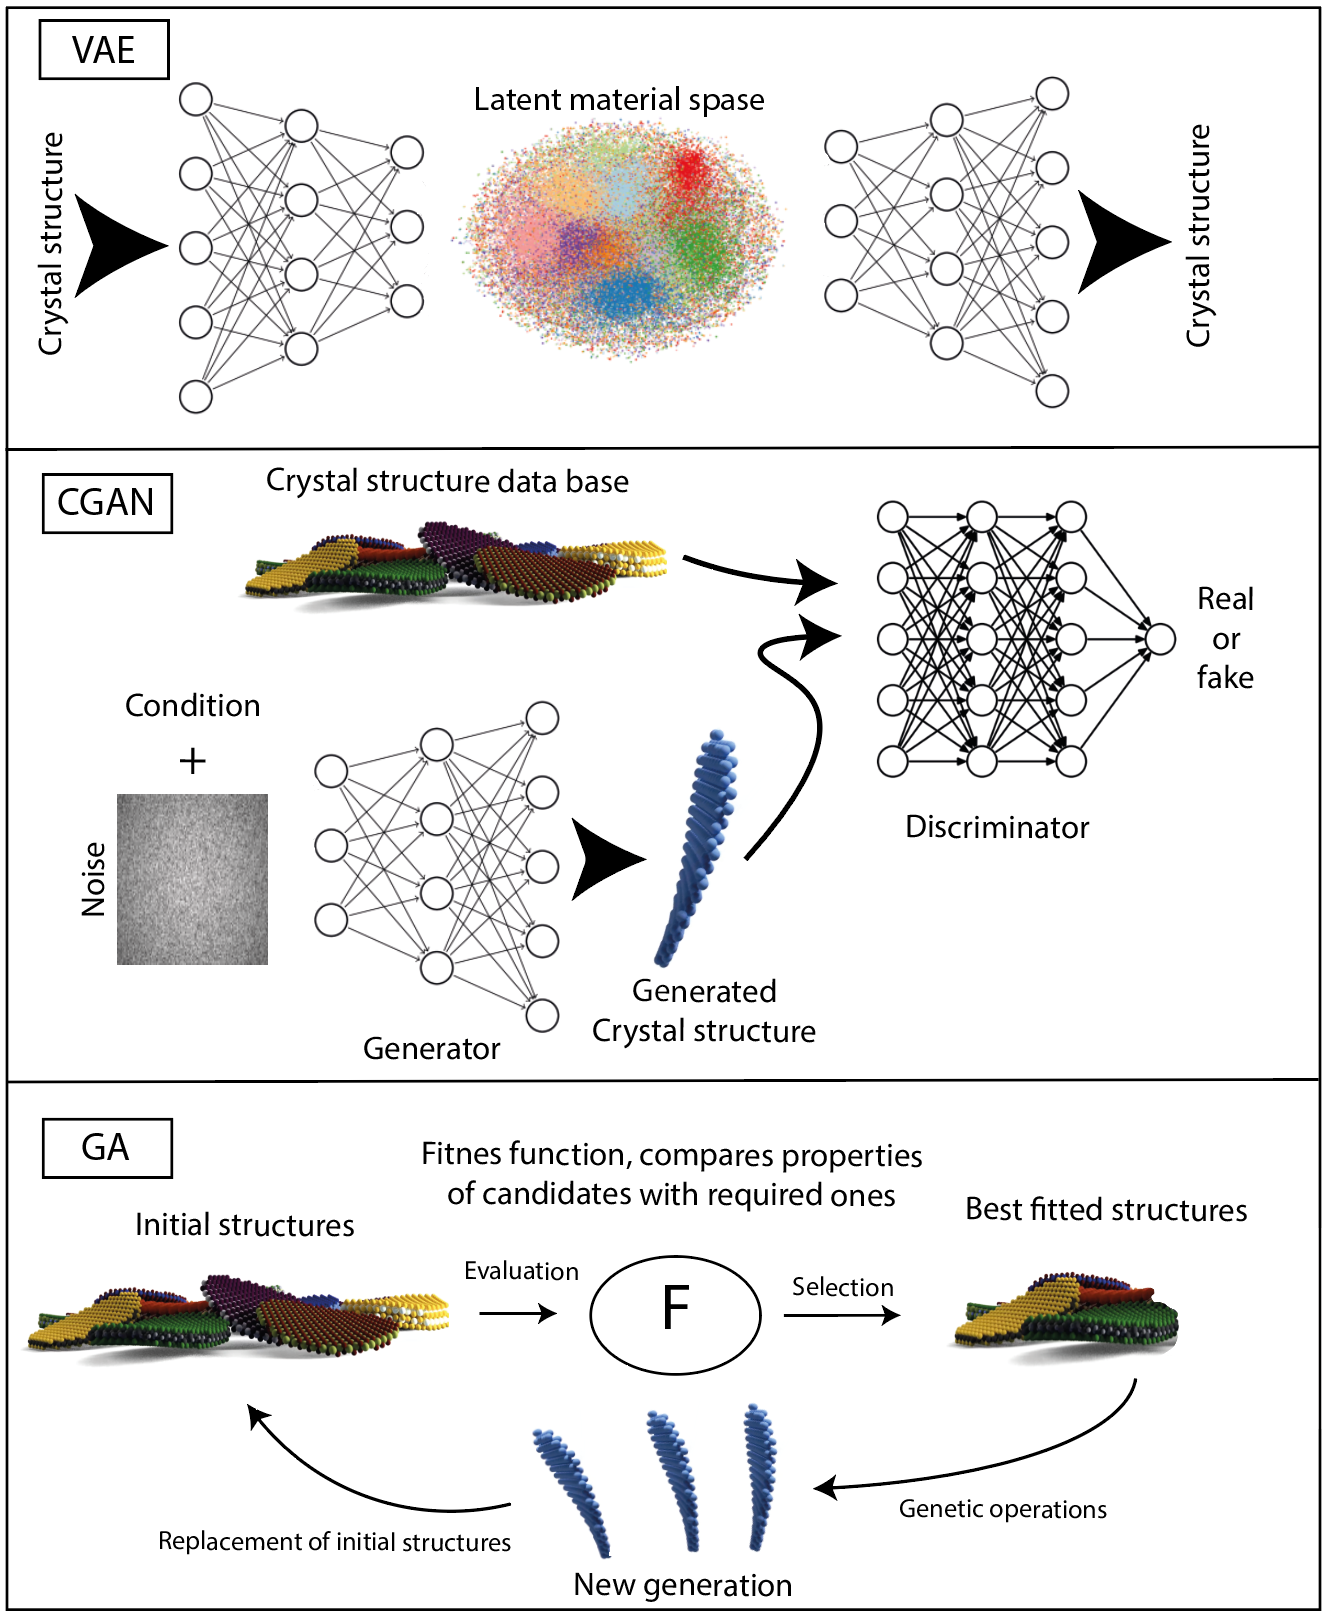
\includegraphics[width=\textwidth]{figures/Generative_models.png}
	\caption{Schematic illustration of VAE, Conditional GAN, and genetic algorithms.}
	\label{fig:generative-models}
\end{figure}

\textbf{Text-based generation}. With the recent explosion of interest in language models (LM), two preprints~\cite{antunes2023crystal, flam2023language} suggest generating material structures as token sequences using Transformer~\cite{vaswani2017attention}. They try two modes: with character-level tokenization, the model generates structures as text files, character-by-character. With atom+coordinate-level tokenization, the model discretizes the atomic coordinates, and uses the resulting bins as coordinate tokens, and generates them together with atom type tokens. The authors claim performance comparable to physically-motivated state-of-the-art models, for generating both crystals and organic molecules. The LM don't respect any kind invariance (permutation, translation, rotation), which makes these ongoing developments even more fascinating. Was the problem that simple all along?

% Bayesian optimization \cite{yamashita2018crystal}
\subsubsection{Reinforcement Learning}
\label{subsec:Reinforcement}

\begin{figure}[H]
    \noindent
    \centering
    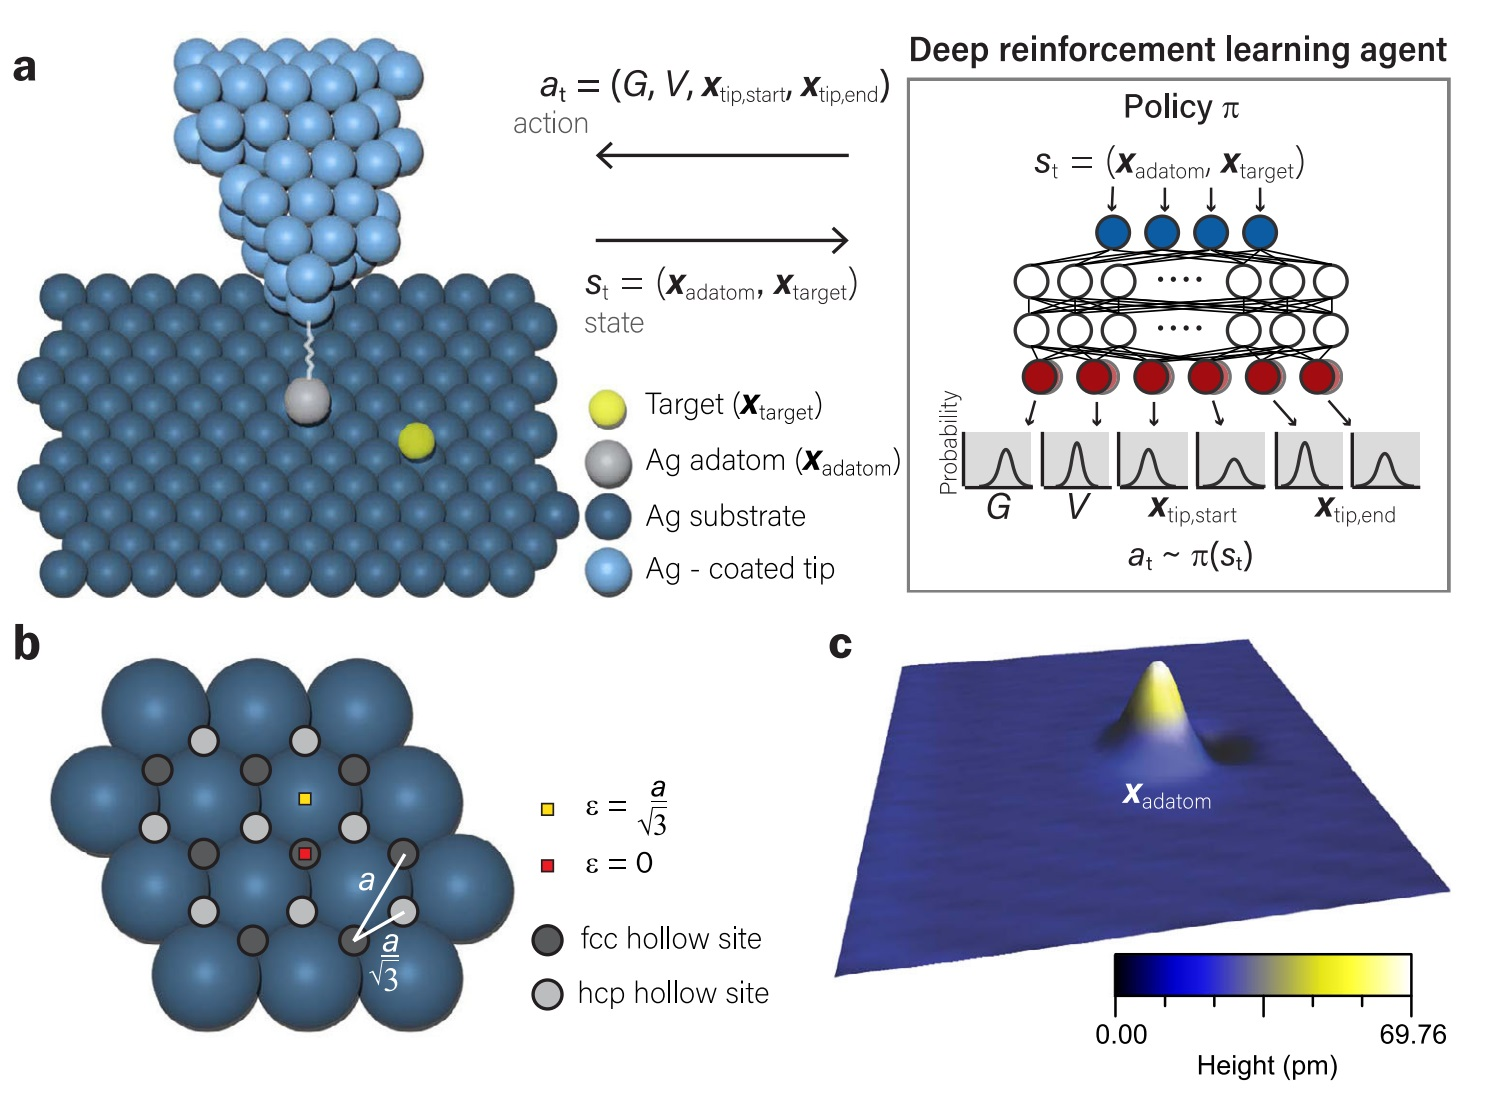
\includegraphics[width=10.6cm]{figures/RL_example.jpg}
    \caption{(a) The RL agent learns to manipulate atoms precisely and efficiently through interacting with the STM environment. STM is operated via actions (commands) $a_t$ consisting of conductance $G$, bias $V$, and the two-dimensional tip position at the start and end of the manipulation $\bm{x}_\text{tip, start}$, $\bm{x}_\text{tip,end}$, which are used to move the STM tip to try to move the adatom to the target position. The agent samples the actions from a distribution (the so-called policy) $\pi(\text{st})$, where it is the state vector consisting of the current and target adatom positions. The policy $\pi$ is modeled as a multivariate Gaussian distribution with mean and covariance given by a neural network. (b) The atom manipulation goal is to bring the adatoms close to the target position as possible. (c) STM image of an \ce{Ag} adatom on \ce{Ag} substrate. Taken from ~\cite{chen2022precise}}
    \label{fig:rl}
\end{figure}

Reinforcement learning (RL) \cite{mousavi2018deep} is one of the machine learning methods during which the model (so-called agent) learns to achieve a goal. Unlike supervised learning, which relies on a static dataset for training, RL is characterized by an agent interacting with a dynamic environment, learning from the consequences of its actions through a trial-and-error strategy. RL methods are widely used in robotics and automated systems. Together with modern achievements in robotics, they allow for automatic
atomically precise material construction, and opens up a way to inverse material design on the surface.

Chen et al. \cite{chen2022precise} propose to use an RL-assisted experimental method to build atom-by-atom \ce{Ag} patterns on a \ce{Ag(111)} surface. The method is further described in figure~\ref{fig:rl}. The interaction of the tip and the atoms is difficult to describe theoretically with sufficiently accurate prediction, and RL allows us to automatically learn the manipulation of specific adatoms with a specific STM machine experimentally.

Banik et al. \cite{banik2021learning} use an RL method to search for optimal defect patterns in \ce{MoS2}. The study proposes to use Monte Carlo Tree Search to explore the defect configuration space and identify potentially stable configurations and evolution paths towards them. 

\subsubsection{Simulation-based inference}
Simulation-based or likelihood-free inference methods are used in various scientific domains to infer the underlying parameters of complex systems. This complexity may stem from a generative or simulating process. However, inferring these parameters poses a significant challenge due to the intractability of the likelihood function (a mapping from observed data to parameters) and the necessity to align simulation model parameters with prior knowledge derived from domain expertise and empirical data. Bayesian inference tackles this challenge by furnishing a framework for inverting simulations.

The typical intractability of the likelihood of observed data given parameters, a vital component for statistical inference, renders traditional statistical methods inapplicable. In simulation-based inference, the statistical model is defined by the simulator itself, with parameters in the model that describe the underlying mechanism and influence the transition probabilities. Moreover, latent variables are integral to the simulation, and the structure of the latent space may vary among simulators.

Various approaches can be used to utilize simulation-based inference for materials design. These approaches share common components: the simulator (e.g DFT algorithms), proposed distribution, and inference method. The simulator's parameters are drawn from the proposal distribution, and the simulator's output is either used directly or as input for a surrogate model, subsequently employed for inference.

There are two broad categories of inference techniques: those that utilize the simulator directly during inference (e.g., approximate Bayesian computation \cite{10.1214/aos/1176346785, alsing2018massive, charnock2018automatic}) and those that construct a surrogate model for inference. The former compares the simulator output directly to the data, while the latter trains a surrogate model using the simulator's output as training data for the estimation or machine learning stages \cite{brehmer2020mining, cranmer2015approximating, stoye2018likelihood}. The relationship between the latter category and generative models is explored in the works of \citet{mohamed2016learning, louppe2019adversarial}.

In Bayesian inference, the ultimate goal is to obtain the posterior distribution of the parameters. Some methods provide samples of parameter points from the posterior, while others yield a tractable function approximating the posterior. The decision on which quantities to infer can be made early or postponed, depending on the method used.

In the probabilistic programming paradigm \cite{le2017inference}, the simulator is written in a probabilistic programming language. Utilizing a probabilistic programming language allows for sampling from the posterior distribution of input parameters and latent variables given observed data. These techniques, based on Markov chain Monte Carlo (MCMC) or training a neural network for proposal distributions, differ from ABC in that the inference engine controls all steps in program execution and biases each draw of random latent variables to enhance the simulation's likelihood of matching observed data, thereby improving sample efficiency. These algorithms facilitate not only the inference of input parameters, but also the entire latent process leading to a specific observation.

Simulation-based inference can be utilized in materials design, offering insight into material properties and performance under various conditions, thereby informing the design process. For a more comprehensive analysis, \citet{cranmerFrontierSimulationbasedInference2020a} provides an excellent review of simulation-based inference.

\subsection{Inverse problem in natural sciences}
One of the earliest examples of an inverse problem is the determination of the shape of a hill from the travel time of a sliding particle on that hill \cite{JournalFurReine}, which was solved by Niels Henrik Abel in 1826 \cite{abazarInverseOptimalControl2020, kellerInverseProblems1976, yamanSurveyInverseProblems2013, groetschIntegralEquationsFirst2007}. This work is generally accepted as the first formal mathematical solution to the inverse problem. However, unlike Abel's problem, which can be solved analytically, many inverse problems are difficult to solve analytically due to their complexity and ill-posed nature. In these cases, different numerical methods are used to approximate the solution by incorporating assumptions and inductive biases in the form of priors and regularizers to restrict the solution space \cite{Jin2010HierarchicalBI, De2007Inverse, Haber2008NumericalMF}.

The inverse problem in non-destructive testing (NDT), which involves determining the specimen parameters based on the response signal from an NDT probe \cite{Udpa1986ADO, Bilicz2012Solution, Blitz1983Nondestructive, Langenberg1997Applied, RNondestructive}, has studied the various techniques and applications of NDT.

In the medical field, inverse problem solutions have a wide range of applications, including medical imaging to construct images of internal tissue structures and diagnose diseases \cite{Aghajani2013ultrasound, Burger2013Inverse, Monard2012Taming, NINVERSE, SComputational, Senouf2019Self, songSolvingInverseProblems2022}, radiation therapy \cite{Alfonso2012class, Bertuzzi2012Optimal, BumanApplications, Hindi2013tutorial, Jalalimanesh2017Multi}, and cardiology as a part of computational fluid dynamics to model fluid flow based on pressure, velocity, and other measurements \cite{Cotter2009Bayesian, Fernandez2013Some, Fourestey2005Solving, Gregson2015Applications, Imanuvilov2020Inverse}.

In geology, inverse problems are used to infer the interior structure or properties of the Earth in terms of density and magnetism, or earthquake data analysis \cite{Barhen2000Optimization, HInverse, Kim2018Geophysical} by analyzing data from various sources such as seismology, gravity, and magnetometry. This type of analysis can help scientists understand the composition and dynamics of the Earth's interior, which is important for understanding processes such as plate tectonics and volcanic activity.
Additionally, inverse problems are used in astronomy to infer information about the properties of celestial objects and the universe based on measurements of electromagnetic waves, such as light and radio waves \cite{Brown1995InversePI}. These techniques can be used to study a wide range of astronomical phenomena, such as the structure of stars \cite{Bellinger2018InversePI, Tsui2006DeterminationOT}, the distribution of matter in galaxies \cite{Daza2020RelationshipBR, Lanusse2013ImagingDM}, and the properties of the cosmic microwave background radiation \cite{Lassas2015OnTI, Lassas2017OnTI}.

In the context of Maxwell inverse design applied to axisymmetric, tunable, and multi-scale metalenses as demonstrated by Rasmus E. Christiansen et al. in \cite{christiansenFullwaveMaxwellInverse2020a} presents a method for fullwave Maxwell inverse design of axisymmetric, tunable, and multi-scale multi-wavelength metalenses. The authors limited the design to an axisymmetric, which allows full-wave Maxwell solvers to be scaled up to structures hundreds or even thousands of wavelengths in diameter, while multilayer topology optimization with tens of thousands of degrees of freedom can tackle more challenging design problems. They also present experimental validation for an axisymmetric inverse-designed monochrome lens in the near-infrared fabricated via two-photon polymerization.

Aberration correction is one of the main challenges for designing metalenses as it is difficult to reduce diffraction along the full optical path. The authors propose an axisymmetric reconstruction technique which reduces the difficulty.

The authors analyze the performances of their design by testing it with various wavelength bands and different focal lengths. They demonstrate that their design is capable of collimating light efficiently over multiple frequencies and distances. It also provides a wide field of view while ensuring an efficient light collection.

The main approaches discussed here involve using the axisymmetric inverse-design method to create reconfigurable lenses that can shift a multifrequency focal spot in response to changes in refractive index, and widely separated multiwavelength lenses (with wavelengths 1 $\mu m$ and 10 $\mu m$). These fullwave Maxwell are solved by discretization using the finite element method \cite{FiniteElementMethod} and solved with COMSOL Multiphysics v5.5 \cite{multiphysics1998introduction}, while also employing the Method of Moving Asymptotes \cite{svanbergMethodMovingAsymptotes1987}, to optimize the multilayer topology with $\approx105$ degrees of freedom, for which the sensitivities of the figures of merits are computed using adjoint sensitivity analysis \cite{lalau-keralyAdjointShapeOptimization2013}.

Computational inverse design is used to design ultra-compact single-piece meta-lenses free of chromatic and angular aberration. Using full Maxwell topology optimization \cite{bendsoeTopologyOptimization2004, jensenTopologyOptimizationNanophotonics2011,moleskyInverseDesignNanophotonics2018} based inverse design tools employ gradient-based optimization techniques to explore hundreds to billions of continuous design variables.

Zin Lin et al. in \cite{linComputationalInverseDesign2021} demonstrated designed inverse ultra-compact metalenses. The resulting designs are single-piece unibody nanophotonic plan-achromats, which can focus incoming plane waves at multiple frequencies and angles with a Strehl ratio of above 0.8 (Gold standard for aberration-free imaging)  and an absolute focusing efficiency of $>50\%$. These meta-lenses are only about 10 wavelengths thick and simultaneous focus over a 60° angular range and a $23\%$ spectral bandwidth without suffering chromatic or angular aberration or a plan-achromat At all angles and frequencies. Results demonstrate the ultra-compact multifunctionality that can be achieved by exploiting the full wave physics of sub-wavelength designs and motivate future work on design and fabrication of multilayer meta-optics.

In \cite{roques-carmes3DPrintedInverseDesignedMetaoptics2022} Charles Roques-Carmes et al. present a framework for the inverse design with density-based topology optimization \cite{bendsoeTopologyOptimization2004, jensenTopologyOptimizationNanophotonics2011} of multi-layer meta-optics structures via topology optimization modelled by the full Maxwell equations due to thickness of each layer being a wavelength-scale and occurrence of multiple scattering events between layers. Maxwell's equations are solved with a finite-difference frequency-domain FDFD solver. This optimization problem is set as constrained continuous optimization problem solved using the method of moving asymptotes \cite{svanbergMethodMovingAsymptotes1987} a gradient-based optimization algorithm designed for non-linear programming in general and structural optimization in particular. To ensure the results of the optimization problem are physically feasible a filter-and-project procedure is applied during the optimization process. The authors demonstrate experimentally a two-layer optical concentrator, focusing incident light at five different angles into the same wavelength-scale spot, reaching 200-300 nm feature size closer to the minimum values of the two-photon polymerization machine.

DFT in combination with Maxwell solvers used to simulate the fundamental effect of light-matter interaction. Both methods are an important part of the material design and analysis workflow. However, formally both methods are exact in practice, a number of assumptions have to be applied \cite{aaronsPerspectiveMethodsLargescale2016} to handle large enough structures.


\subsection{Discussion and outlook}
In this article, we review the state of the art in machine learning for material design. The main data-driven methods and their applications for forward and inverse design in materials science were considered. ML methods in the scope of two-dimensional materials have yet to show their full potential. The main limiting factor is the small amount of data available for training models and still huge material search space.

Due to the high computational cost of HTS methods (like DFT), only a fraction of the desired materials and their properties can be directly calculated. However, the situation is changing as the area is attracting more and more attention. Improvement of the HTS methods on one side and constant increase of computational power on another might reveal the option of simulating materials with large unit cells and covering more material properties.

Despite the fascinating progress of deep learning models, such approaches also have certain disadvantages, such as insufficient interpretability of models \cite{gilpin2018explaining}. All large ML models are used as a kind of black box. Furthermore, the generalizability of these models remains a significant concern.

Also, one of the important disadvantages of all results achieved by data-driven approaches is that these results are purely theoretical and have not been presented in comparison with experimental data, and the difference can be significant. Currently, the experimental data are insufficient. Experimentation remains the bottleneck in the problem of material design.

An automated laboratory for searching, synthesizing and testing (measuring) materials would solve this problem of automatizing experimental material search and data acquisition. The first prototypes have already been demonstrated~\cite{burger2020mobile,coley2019robotic}. Production and measurement of 2D materials on demand in a feedback loop with self-correcting ML algorithms will be a game-changing milestone.

Overall, progress in this area shows that the class of two-dimensional materials and their derivatives is little studied, and there are many materials with potentially unique properties that have not yet been synthesized. Everything indicates that in the near future, we will have many discoveries in this area, some of which lie on the surface.
